\part{Global Illumination}
In a single frame in real time, every light source casts thousands of rays (photons) to the scene, some are absorbed, some run out of the scene, and the others go through multiple bounces and reach to the camera forms the final image we seen.

Simulating such process is time-consuming. Technically there are two problems must be solved: First, in a single point of a surface, we must do integral calculation over the hemisphere because a point could receive rays from all other points in the scene; Second, for every ray, we must find the nearest intersection which usually needs to iterate every geometry in the scene. Current generation hardware can not handle these computation in real-time. 

Basically, there are two ways to handle these problems: rasterization and approximation. For avoiding intersection calculation, rasterization iterates every vertex of every mesh in the scene and renders them to the screen space. By using depth tests, the nearest points are kept and the further points are blended. Also for avoiding intersection calculation, rasterization method usually ignores shadows (visibility), which needs to compute the possible intersections between the point and the light source. Rasterization is fast and almost all modern GPUs was designed to support rasterization. 

Rasterization has some problems (or something it doesn't take care). First, rasterization ignores visibility, so we need some other ways to handle shadows; Second, rasterization usually only compute the light comes from the light source directly and ignores the bounced lights, which needs integral calculation, from the others points in the scene. So it's usually called local illumination. We need other ways to compute the bounced lights which is the subject this article will introduce.

Since the main goal is to render a plausible, convincing image, not a physically correct result. We can make some assumptions to approximate the problems. That's the core of many global illumination techniques, such as environment maps assume the light is distant; some techniques assume indirect lighting is low-frequency; In global illumination techniques, we can understand them by knowing how they approximate the results which we will see many in this article.

The main goal of this article is to detail different global illumination methods (other good material can be seen at \cite{a:TheStateoftheArtinInteractiveGlobalIllumination}). These methods are not isolated - some methods are based on others. These connections are very important which help us understand them better and is the second goal.

We first introduced some basic concepts, such as radiometric, rendering equation, BRDF theory, spherical harmonics, etc. Then we will list some phenomena which we must implement in the game. The rest chapters detail some main global illumination methods which have been used widely, from precomputation to real-time techniques.



\chapter{Basis}
\section{Radiometry}
The rendering equation of computer graphics deals with some concepts from radiometry. \textit{Radiometry} is the study of physical measurement of electromagnetic radiation, including visible light. It defines a common terminology for the physical quantities and units that are used by the rendering equation and other algorithms. These quantities can be seen in table \ref{t:radiometric-quantities}.

\begin{table}\label{t:radiometric-quantities}
\centering
	\begin{tabular}{l|l}
  Radiometric Quantity&Units  \\
  \hline
  radiant energy & $J$ \\
  radiant flux & $W$  \\
  irradiance & $W/m^2$ \\
  radiance & $W/(m^2\cdot sr)$
\end{tabular}
\caption{Radiometric quantities and units}
\end{table}

\paragraph{\textbf{Radiant energy}} 
In radiometry, the basic unit is energy or \textit{radiant energy} $Q$, measured in \textit{joules} (abbreviated "J"). Each photon has some amount of radiant energy that is proportional to its frequency $v$.

\begin{equation}
	Q=hv
\end{equation}

where $h$ is Planck's constant ($6.62620\times 10^{-34}$ joule-seconds). In the \textit{visible spectrum}, "bluer" photons are more energetic, and "redder" photons are less energetic.

\paragraph{\textbf{Radiant flux}} or \textit{radiant power}, denoted $\Phi$, expresses the amount of energy flowing across a surface over time, see figure \ref{f:radiometric-quantities}(a). This is the same quantity that is used to describe the power of light bulbs and is expressed in terms of watts[$W=J\cdot s^{-1}$].

\paragraph{\textbf{Irradiance}} is the density of radiant flux with respect to a unit area surface perpendicular to the light direction $\mathbf{l}$, see figure \ref{f:irradiance-measure}. Hence it has units of [$W\cdot m^{-2}$] and can be expressed in terms of flux as: 

\begin{figure}
\sidecaption
	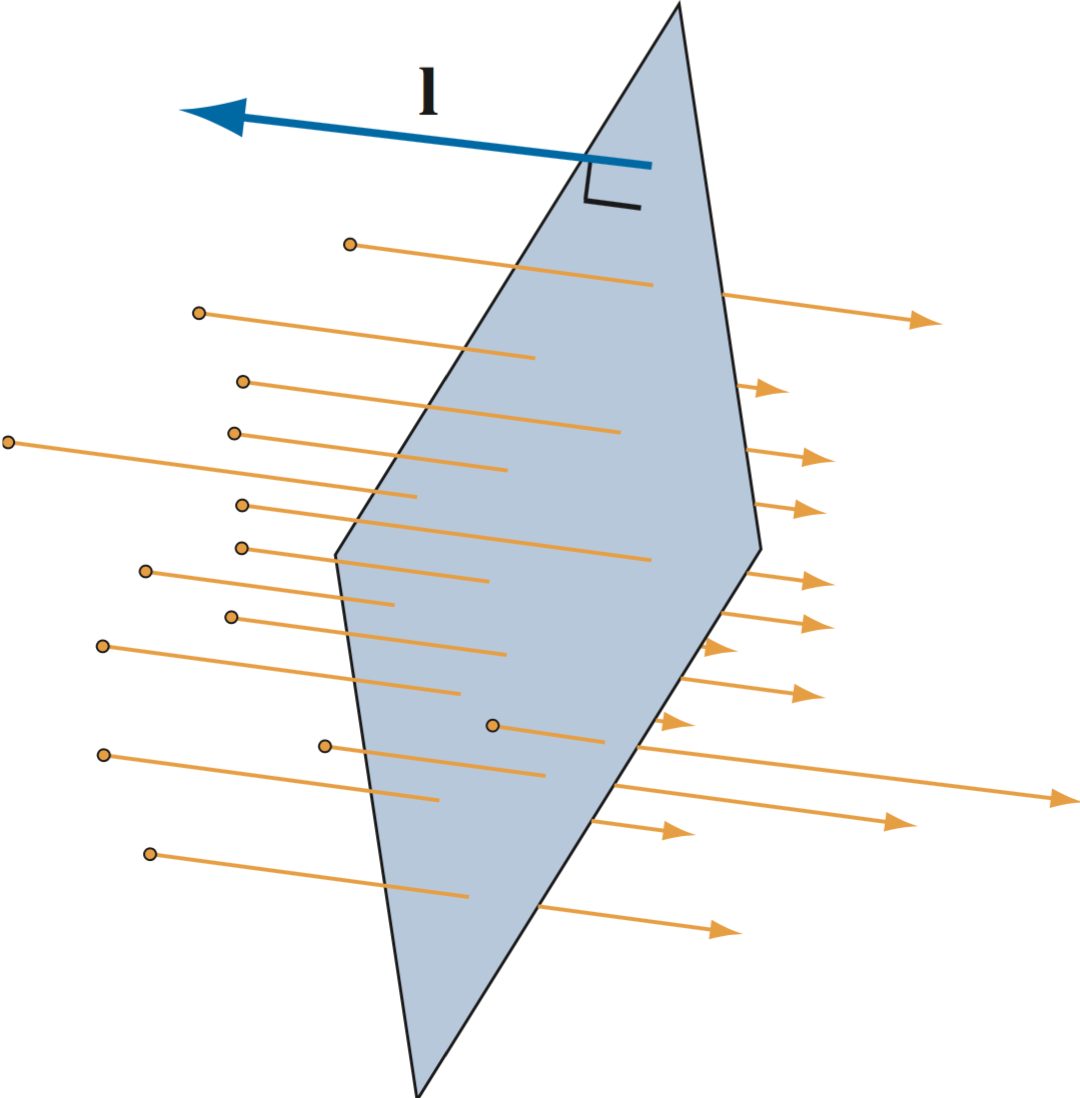
\includegraphics[width=0.5\textwidth]{graphics/gi/irradiance}
	\caption{Measuring the magnitude of light emitted by a directional light source.}
	\label{f:irradiance-measure}
\end{figure}

\begin{equation}
	E=\frac{d\Phi}{dA}
\end{equation}

Irradiance $E$ is used to measure light flowing into a surface and exitance $M$ (also called \textit{rediosity} or \textit{radiant exitance}) is used to measure light flowing out of a surface. The general term \textit{radiant flux density} is sometimes used to refer to both irradiance and exitance.

Although measuring irradiance at a plane perpendicular to $\mathbf{l}$ tells us how bright the light is in general, to compute its illumination on a surface, we need to measure irradiance at a plane parallel to that surface (i.e., perpendicular to the surface normal $\mathbf{n}$). The surface irradiance is equal to the irradiance measured perpendicular to $\mathbf{l}$, times the cosine of the angle $\theta_i$ between $\mathbf{l}$ and $\mathbf{n}$, see figure \ref{f:irradiance-cosine-term}.

\begin{figure}
	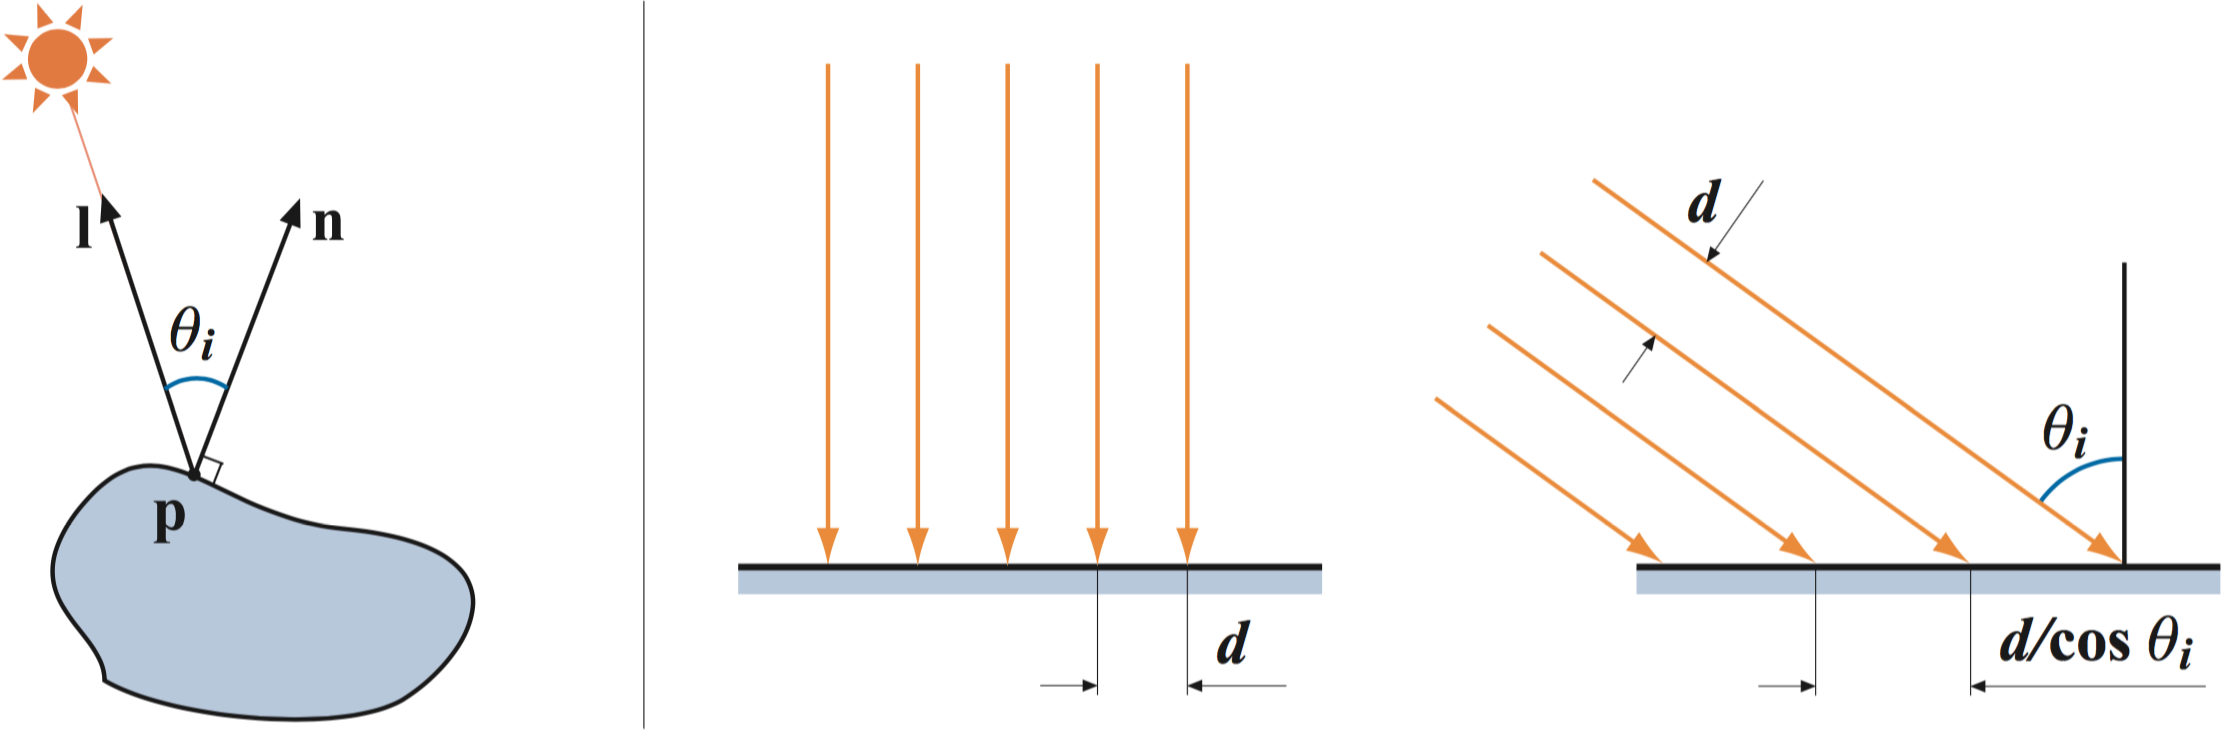
\includegraphics[width=1.\textwidth]{graphics/gi/irradiance-cosine-term}
	\caption{The diagram on the left shows the lighting geometry. In the center, light is shown hitting a surface straight-on, and on the right it is shown hitting the surface at an angle.}
	\label{f:irradiance-cosine-term}
\end{figure}

The center and right illustrations in figure \ref{f:irradiance-cosine-term} show a geometric interpretation of this cosine factor. As $\theta_i$ increases, the same radiant flux goes through a larger area per second, the irradiance of the surface decreases. 

$E$ is used in equations for irradiance, most commonly for irradiance perpendicular to $\mathbf{n}$. We use $E_L$ for irradiance perpendicular to $\mathbf{l}$. Note that a negative value of the cosine corresponds to the case where light comes from below the surface. In this case the light does not illuminate the surface at all, so we will use the cosine clamped to non-negative values (symbolized by $\overline{cos}$):

\begin{equation}
	\begin{aligned}
		E&=E_L \overline{cos}\theta_i\\
		&=E_L max(\mathbf{n}\cdot\mathbf{l},0)
	\end{aligned}
\end{equation}

This cosine factor is very important in the rendering equation. And it can be easily computed in a shader by taking the dot product of the two vectors (note that both $\mathbf{l}$ and $\mathbf{n}$ are always assumed to be of length 1). 

\begin{figure}
\sidecaption
	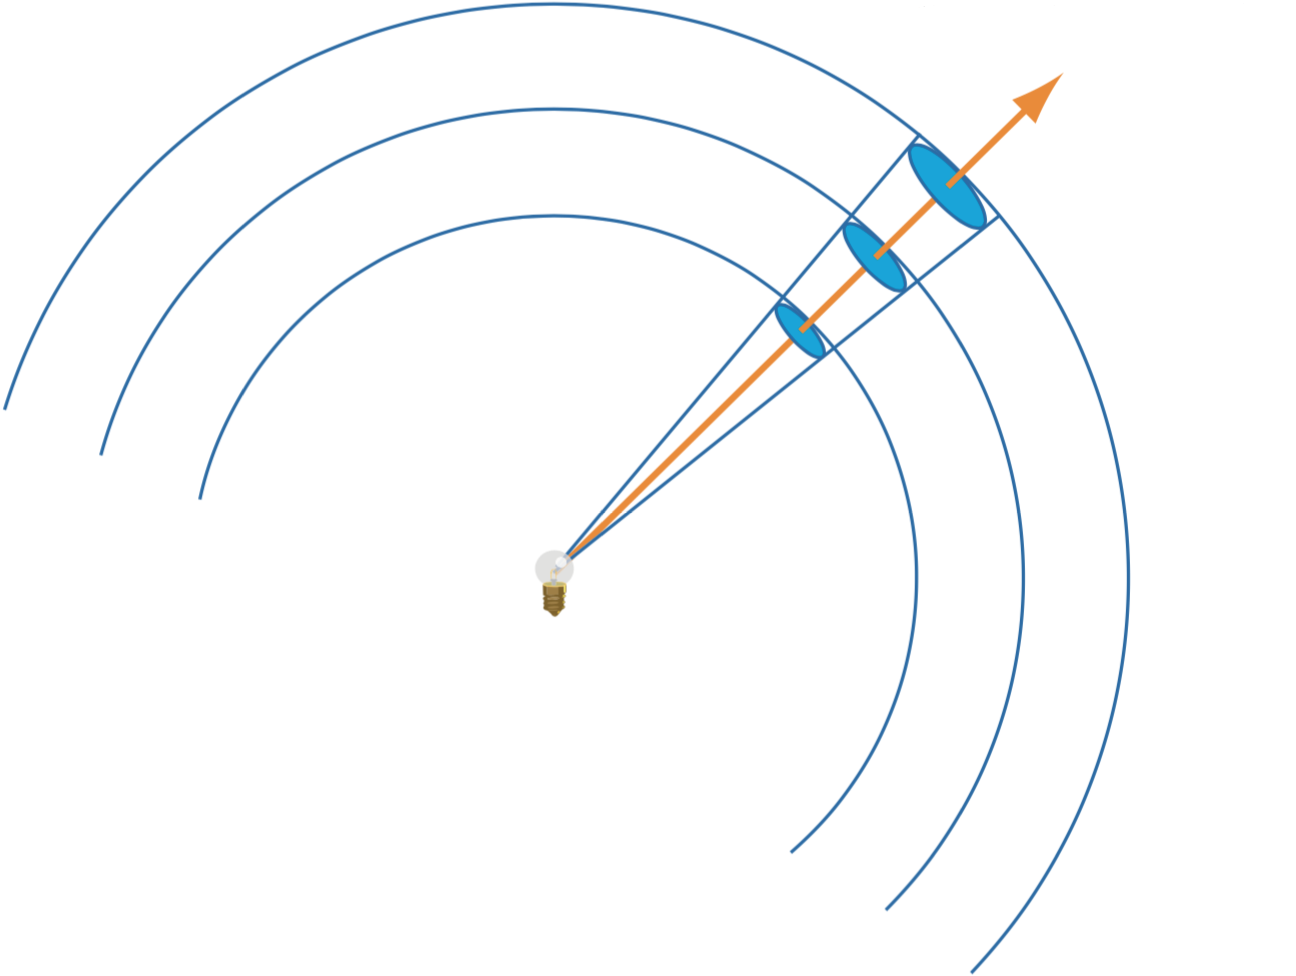
\includegraphics[width=0.5\textwidth]{graphics/gi/radiance}
	\caption{$E_L$ varies with distance.}
	\label{f:radiance}
\end{figure}

\paragraph{\textbf{Radiance}} For closer light sources, $E_L$ varies with distance and can not be treated as a constant (directional light). Imagine concentric spheres around the light bulb, see figure \ref{f:radiance}.  We want to examine the light emitted in a particular direction (the orange arrow). But first we need to define what is a direction.

An angle is a set of directions in a plane, and its size in radians is equal to the length of the arc it intersects on an enclosing radius-1 circle. An angle of $2\pi$ radians covers the whole unit circle. Extending this to three dimensions, a \textit{solid angle}, denoted $\omega$, is a continuous set of directions, measured with \textit{steradians} (abbreviated "sr"), which are defined by patch area on a radius-1 sphere. A solid angle of $4\pi$ steradians would cover the whole area of the unit sphere. See figure \ref{f:solid-angle}.

\begin{figure}
\sidecaption
	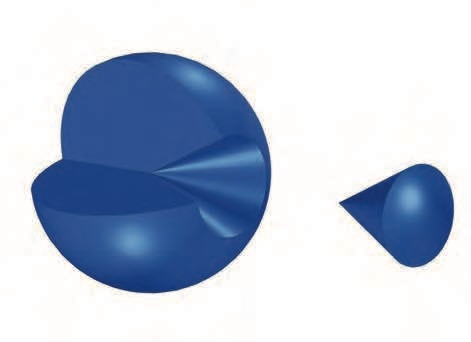
\includegraphics[width=0.65\textwidth]{graphics/gi/Steradian}
	\caption{A cone with a solid angle of one steradian removed from a cutaway view of a sphere. The shape itself is irrelevant to the measurement; the coverage on the sphere's surface is the key.}
	\label{f:solid-angle}
\end{figure}

\textit{Radiance} measures the illumination in a single ray of light--it is flux density with respect to both area and solid angle. The metric units of radiance are [$W/m^2 \cdot sr$]. Radiance is:

\begin{equation}
	L=\frac{dE_{proj}}{d\omega}=\frac{d^2 \Phi}{dA_{proj}d\omega}
\end{equation}

Radiance $L$ is what sensors (such as eyes or cameras) measure, so it is of prime importance for rendering. The purpose of evaluating a shading equation is to compute the radiance along a given ray (from the shaded surface point to the camera).


\section{Interaction of Light with Surfaces}
To formulize the rendering equation, we need to understand how light interact with surfaces. the basic relevant physical phenomena can be described as:

\begin{itemize}
	\item Light is emitted by the sun or other sources.
	\item Light interacts with objects in the scene; part is absorbed, part is scattered and propagates in new directions.
	\item Finally, light is absorbed by a sensor(human eye, electronic sensor, or film).
\end{itemize}

This process involves three components: light source, surface and camera. We have known that irradiance can be used to represent a light source energy distribution, and radiance can be used to describe the incident light of a point. This section, we will detail the interaction of light with surfaces.

\subsection{Geometric (Ray) Optics}

The theory of optics is very complicated. In computer graphics, we make some assumptions about the behavior of light that limit the types of phenomena that can be simulated, that is:

\begin{itemize}
	\item Light can only be emitted, reflected and transmitted.
	\item Light is assumed to travel in straight lines and at infinite speed.
\end{itemize} 

\begin{figure}
\sidecaption
	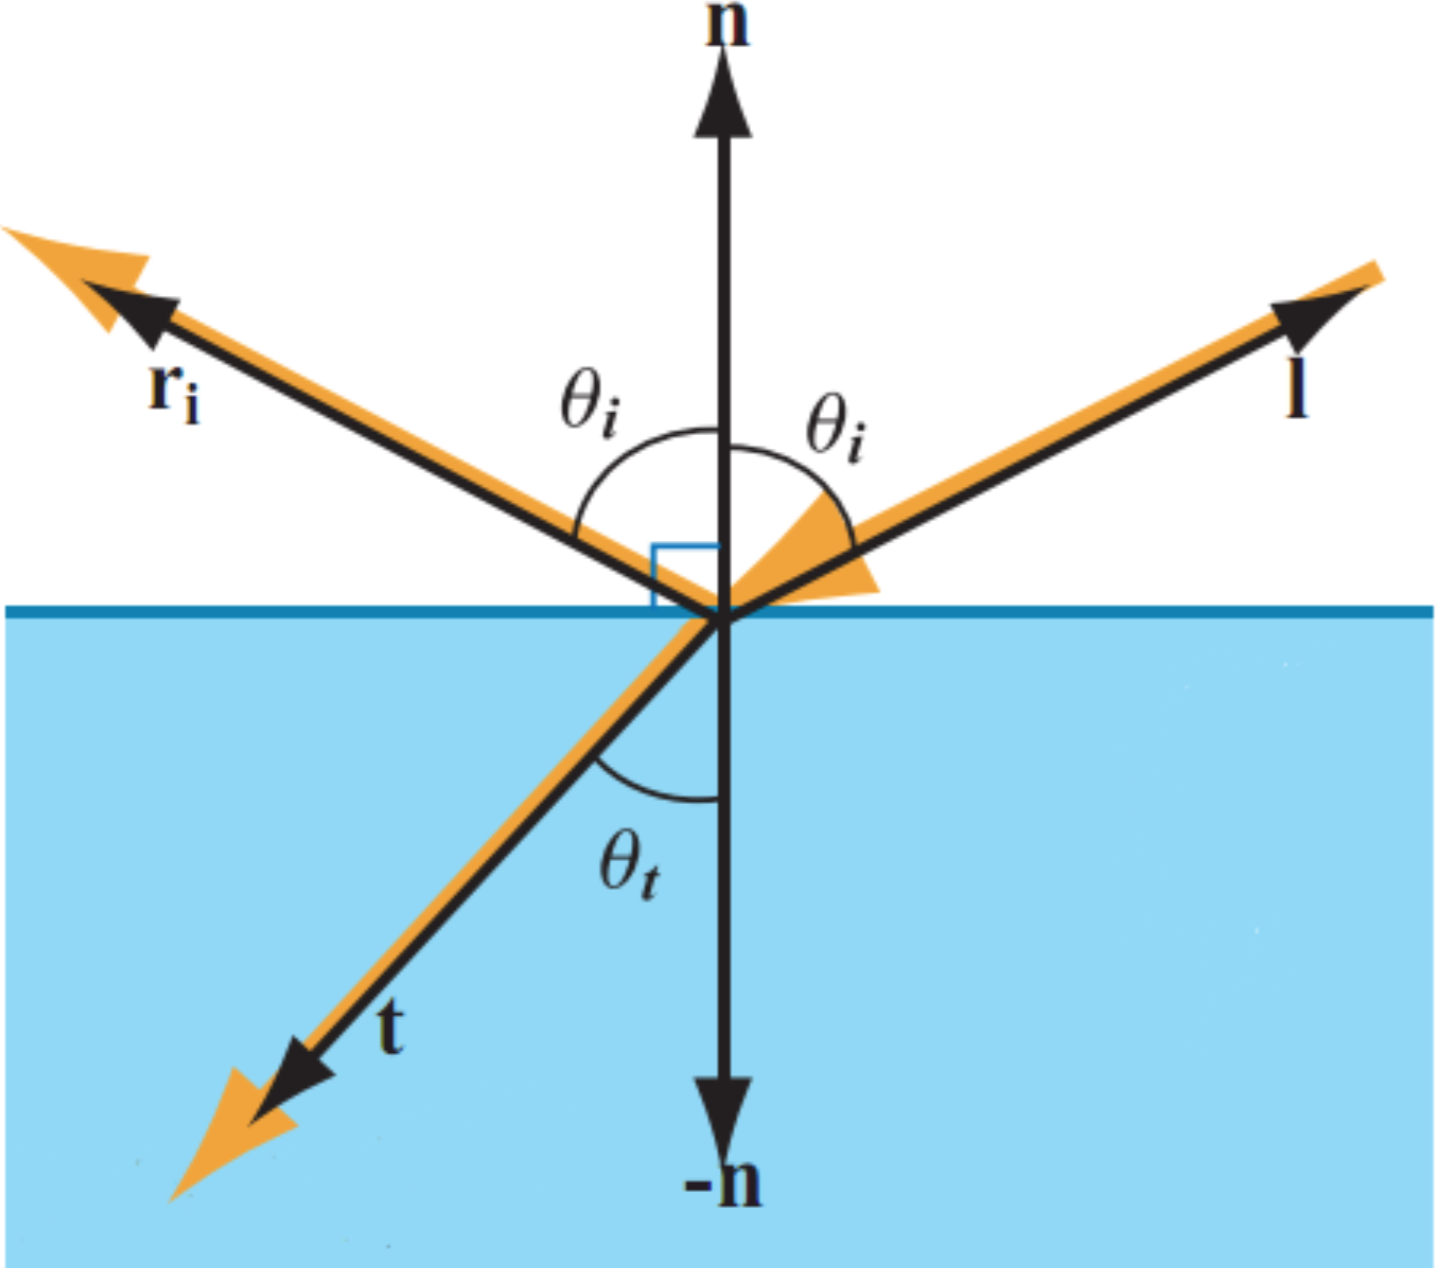
\includegraphics[width=0.65\textwidth]{graphics/gi/ray-optics-1}
	\caption{The Law of Reflection and Snell's Law determine reflection and refraction.}
	\label{f:Ray-optics-model}
\end{figure}

This model is called \textit{Geometric} or \textit{ray optics}. In this model, we will treat optically smooth surfaces as being perfectly flat. With such surfaces, the direction of the reflected ray is determined by the Law of Reflection: given incident ray $\mathbf{l}$ and surface normal $\mathbf{n}$, the incident and reflected rays lie in a single plane, and the angle between the reflected ray and the surface normal, is the same as that between the incident ray and the normal. see figure \ref{f:Ray-optics-model}.

When light travels through an area of space that has a changing index of refraction, refraction occurs. When there is an interface between a uniform medium with index of refraction $n_1$ and another medium with index of refraction $n_2$. In such situations, Snell's Law describes the resulting deflection of the light ray:

\begin{equation}
	n_1\sin\theta_1 = n_2\sin\theta_2\ 	
\end{equation}

\begin{figure}
\sidecaption
	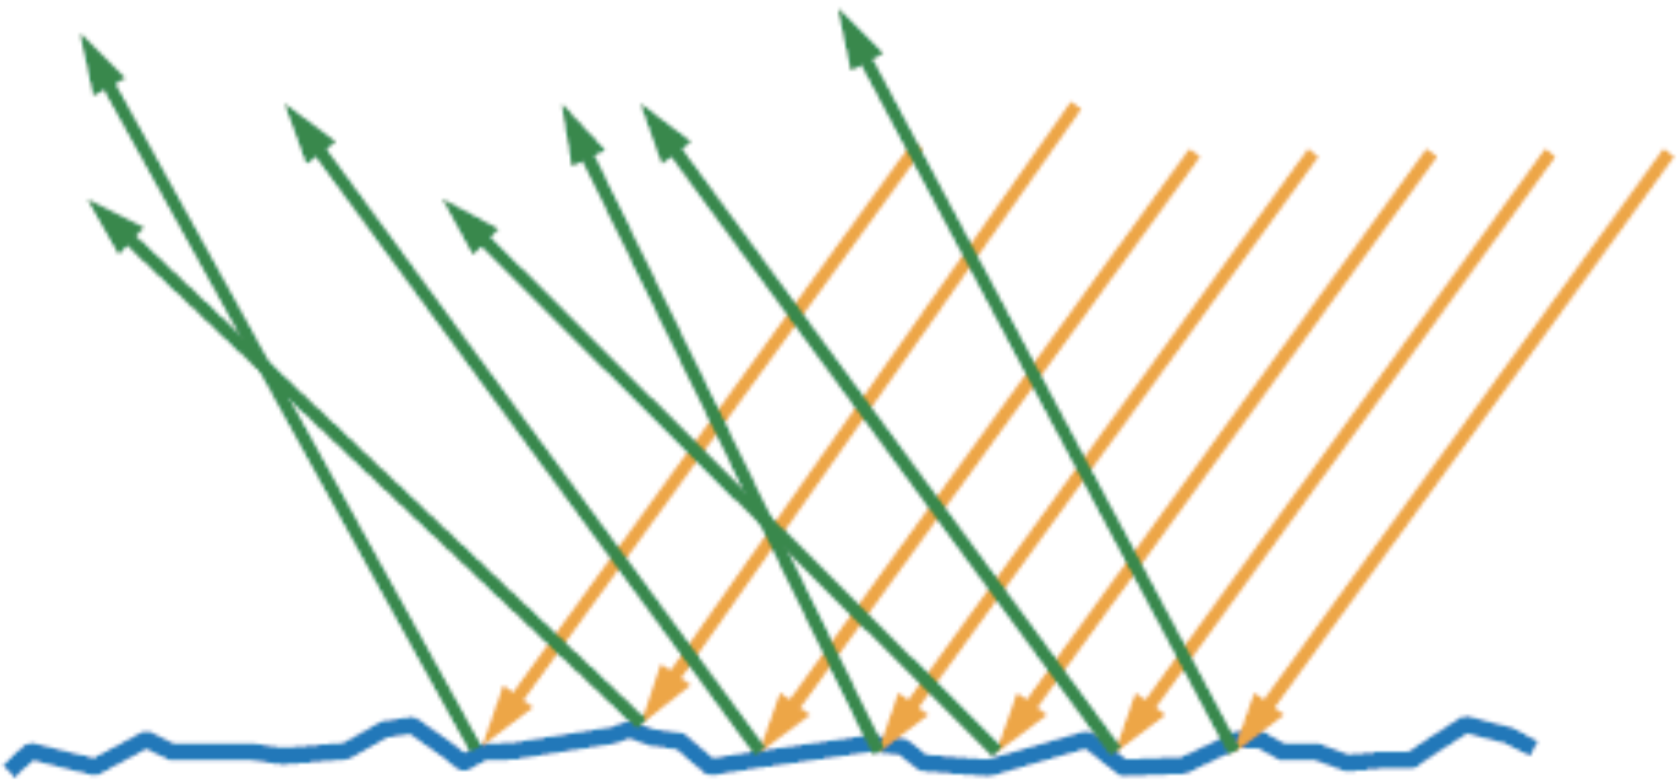
\includegraphics[width=0.65\textwidth]{graphics/gi/ray-optics-3}
	\caption{This microgeometry variation causes each surface point to reflect (and refract) light in a different direction.}
	\label{f:microgeometry}
\end{figure}

Most real-world surface are not optically smooth but possess irregularities at a scale much larger than a light wavelength, but smaller than a pixel. This microgeometry variation causes each surface point to reflect (and refract) light in a different direction, see figure \ref{f:microgeometry}.

As a result, a single incident ray will be reflected (or refracted) into multi-directions, which equals from a given view direction, we could see multi-incident rays, see figure \ref{f:multi-rays}. As we will see in the next subsection, the smoothness (or roughness) of the surface can determine how large directions the incident rays can be reflected or refracted, see figure \ref{f:roughness}.

\begin{figure}
\sidecaption
	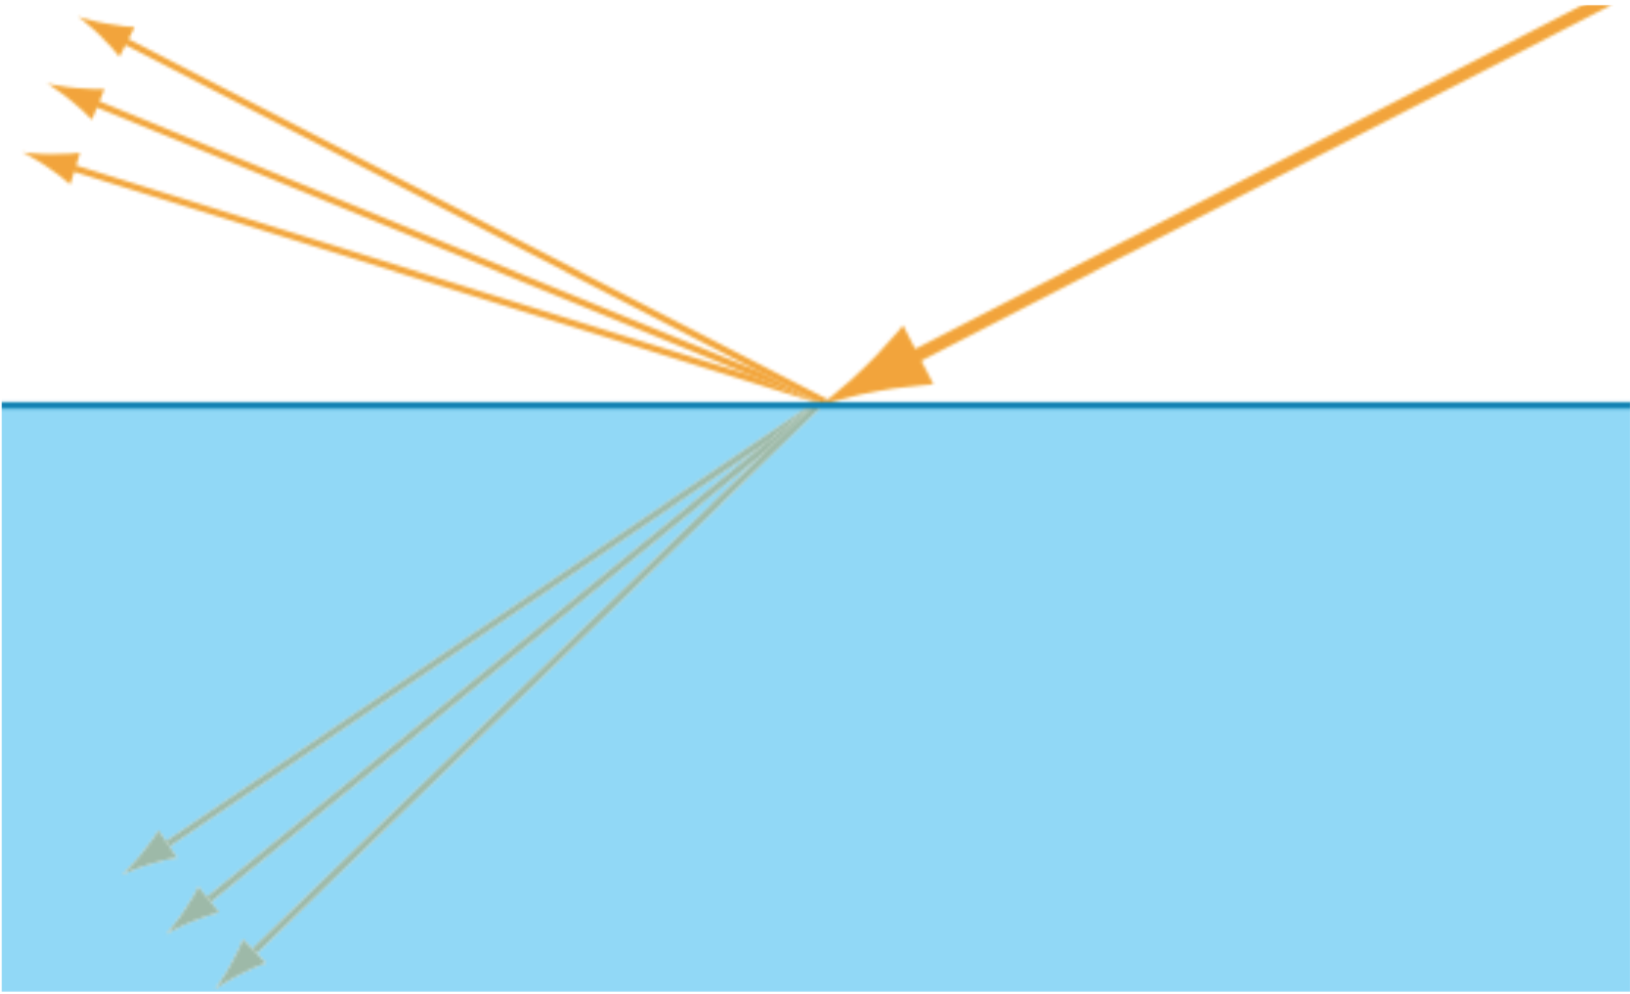
\includegraphics[width=0.65\textwidth]{graphics/gi/ray-optics-4}
	\caption{This microgeometry variation causes each surface point to reflect (and refract) light in a different direction.}
	\label{f:multi-rays}
\end{figure}

What happens to the refracted light? It depends on what kind of material the object is made of. In computer graphics, materials can be grouped into two categories: metals and non-metals. Metals immediately absorb all refracted light.

\begin{figure}
\sidecaption
	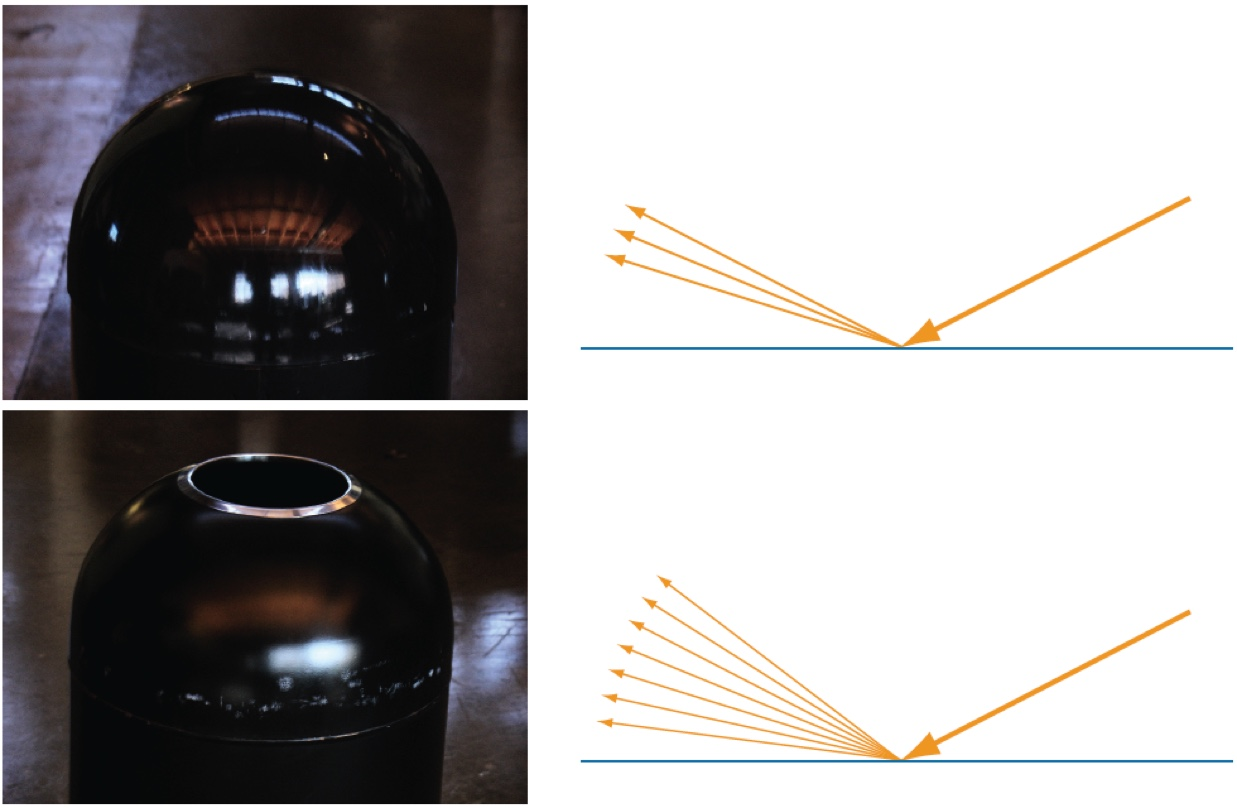
\includegraphics[width=0.65\textwidth]{graphics/gi/ray-optics-2}
	\caption{The rougher the surface, the wider the cones of reflected and refracted directions will be.}
	\label{f:roughness}
\end{figure}

For non-metals, refracted light is scattered and/or absorbed to some degree. Unless the object is made out of a clear substance like glass or crystal, there will be enough scattering that some of the refracted light is scattered back out of the surface: these are the blue arrows you see coming out of the surface in various directions. see figure \ref{f:refraction}.

\begin{figure}
\sidecaption
	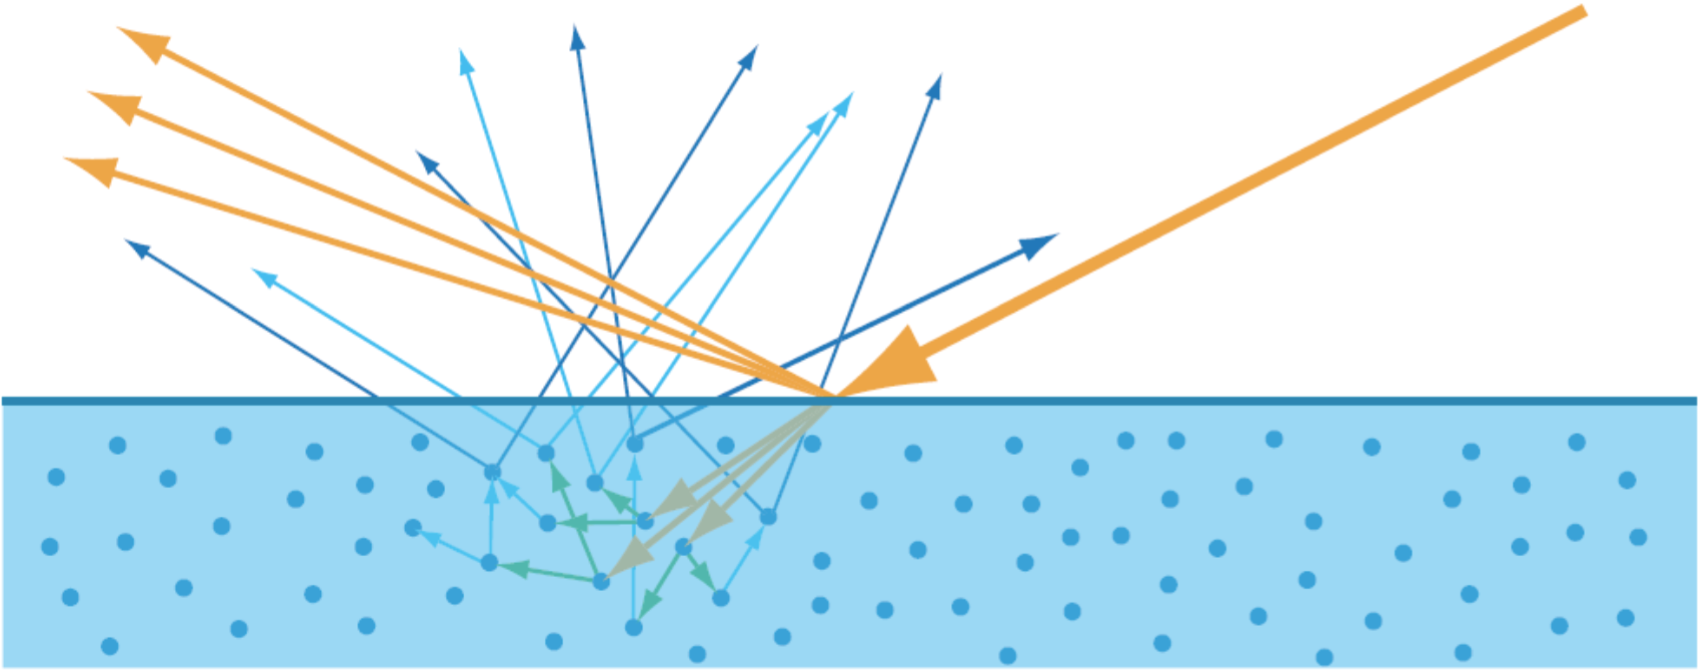
\includegraphics[width=0.65\textwidth]{graphics/gi/ray-optics-5}
	\caption[][21mm]{In non-metal materials, the refracted light will be re-emitted back to the air after enough scattering.}
	\label{f:refraction}
\end{figure}

The distribution of distances between the re-emitted point and the entry depends on the property of the surface. If the pixel size is large compared to the entry-exit distances, we can assume that the distance are effectively zero for shading purpose, and it's called \textit{local subsurface scattering}. Otherwise it's called \textit{global subsurface scattering}. We only discuss local subsurface scattering in this article. 

\begin{figure}
\sidecaption
	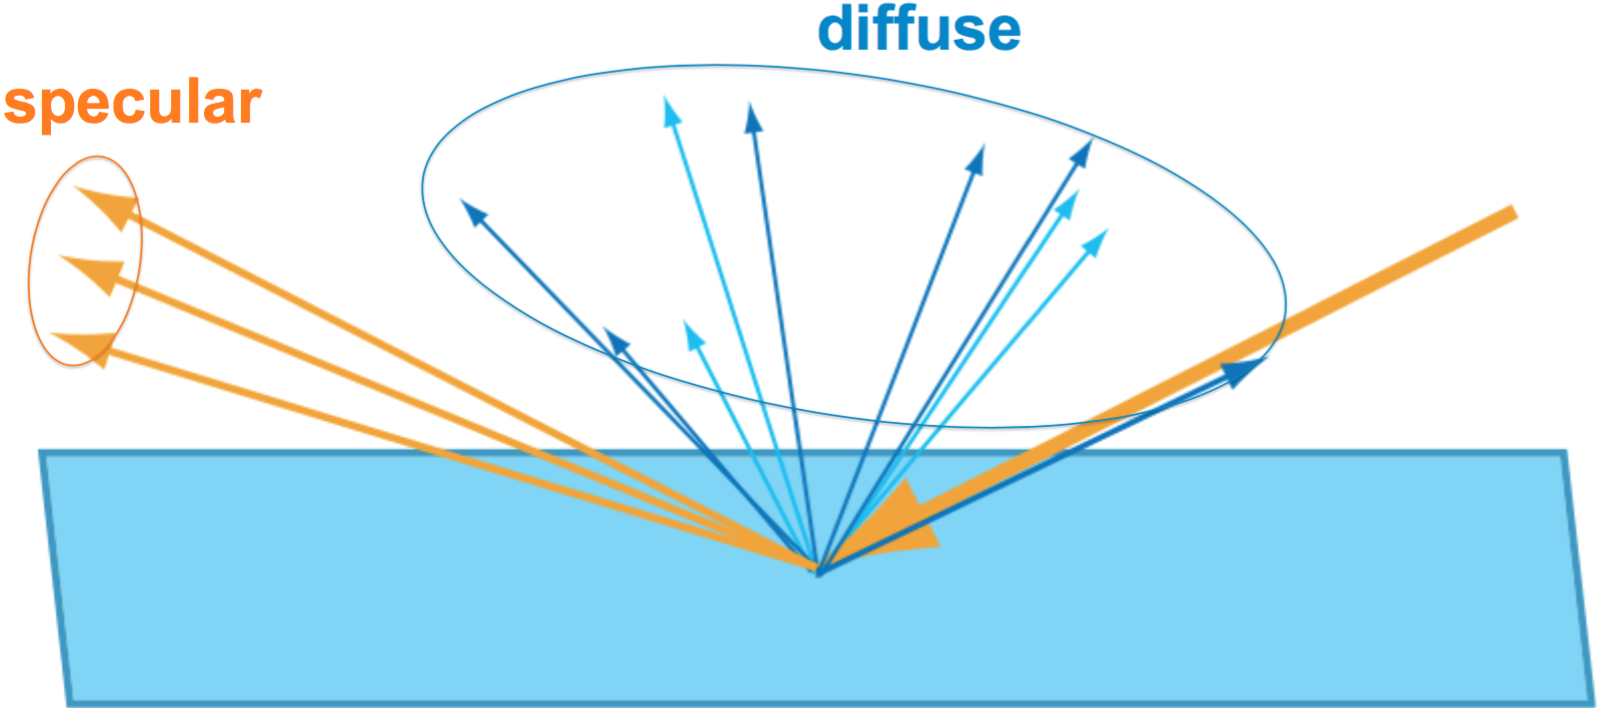
\includegraphics[width=0.65\textwidth]{graphics/gi/ray-optics-6}
	\caption{Light interactions are split into "specular" and "diffuse" term.}
	\label{f:specular-and-diffuse}
\end{figure}

It is convenient to split these two very different light-material interactions into different shading terms. We call the surface reflection term "specular" and the term resulting from refraction, absorption, scattering, and re-refraction we call "diffuse", see figure \ref{f:specular-and-diffuse}.

We have discussed the physics of light/matter interactions. Next subsection we will turn these physics into mathematical models that can be used for shading.



\subsection{BRDF}
How does exactly these reflected or refracted directions distribute mathematically? The answer is \textit{bidirectional reflectance distribution function}, or \textit{BRDF}. The precise definition of BRDF is the ratio between differential outgoing radiance and differential irradiance:

\begin{equation}
	f(\mathbf{l},\mathbf{v})=\frac{dL_o(\mathbf{v})}{dE(\mathbf{l})}
\end{equation}

which is a function of light direction $\mathbf{l}$ and view direction $\mathbf{v}$, see figure \ref{f:brdf}. 

\begin{figure}
	\sidecaption
	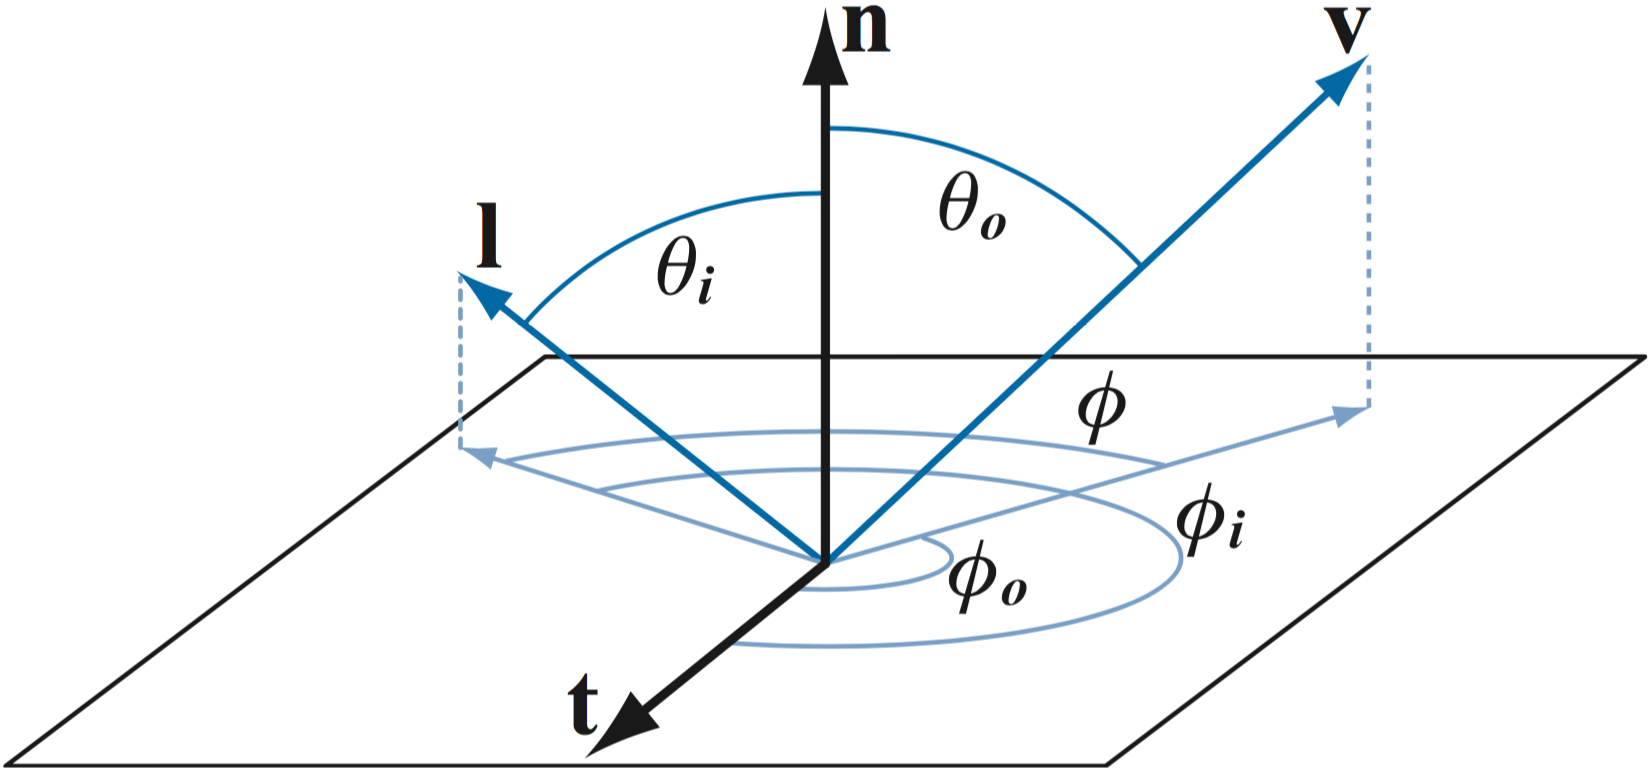
\includegraphics[width=0.65\textwidth]{graphics/gi/ray-optics-7}
	\caption{The BRDF. Azimuth angles φi and φo are given with respect to a given tangent vector t. The relative azimuth angle φ (used for isotropic BRDFs instead of φi and φo) does not require a reference tangent vector.}
	\label{f:brdf}
\end{figure}

Given BRDF, the outgoing radiance from a point equals the integral of incoming radiance times BRDF times a cosine factor (we've seen in the previous section), over the hemisphere of incoming direction:

\begin{equation}\label{e:reflectance}
	L_o(\mathbf{v})=\int_{\Omega}f(\mathbf{l},\mathbf{v})\otimes L_i(\mathbf{l})(\mathbf{n}\cdot\mathbf{l})d\omega_i
\end{equation}

the $\otimes$ notation means component-wise RGB multiplication. The equation \ref{e:reflectance} is called the \textit{reflectance equation}.

\subsubsection{BRDF Characteristics}
The laws of physics impose two constrains on any BRDF.

\paragraph{\textbf{Helmholta reciprocity}} which means that the input and output angles can be switched and the function value will be the same:

\begin{equation}
	\begin{aligned}
		f(\mathbf{l},\mathbf{v})&=f(\mathbf{v},\mathbf{l}) \text{,  or  }\\
		f(\mathbf{x},\vec{\omega}^{'},\vec{\omega})&=f(\mathbf{x},\vec{\omega},\vec{\omega}^{'})
	\end{aligned}
\end{equation}

In practice, BRDFs used in rendering often violate Helmholtz reci- procity without noticeable artifacts. However, it is a useful tool to use when determining if a BRDF is physically plausible.

Because of this property, we use the following notation for the BRDF to indicated that the directions can be interchanged:

\begin{equation}
	f(\mathbf{x},\vec{\omega}^{'},\vec{\omega})
\end{equation}

From a practical point of view, reciprocity means that surface reflection is invariant to the direction of light flow, i.e, the reflected radiance remains unchanged if the light and camera positions are swapped. This property is essential for many global illumination algorithms and allows light to be traced either in the forward or backward direction.


\paragraph{\textbf{Conservation of energy}} which means the out going energy con not be greater than the incoming energy. This can be expressed as the following:

\begin{equation}
	\int_{\Omega}f(\mathbf{x},\vec{\omega}^{'},\vec{\omega})(\vec{\mathbf{n}}\cdot\vec{\omega}^{'})d\vec{\omega}^{'}\leq 1, \forall\vec{{\omega}}
\end{equation}

For real-time rendering, strict energy conservation is not necessary, but approximate energy conservation is desirable. A surface rendered with a BRDF that grossly violates energy conservation might look much too bright, decreasing realism.


\subsubsection{Visualizing BRDF}
Due to BRDF obey the law of physics (reciprocity and energy conservation), the rendering follows BRDF is sometimes called \textit{physically based shading}. To design you BRDF model, It is very important to visualize it, see figure \ref{f:brdf-models}.

\begin{figure}\label{f:brdf-models}
\begin{center}
	\begin{subfigure}[b]{0.325\textwidth}
		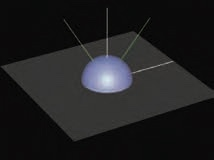
\includegraphics[width=1.\textwidth]{graphics/gi/ray-optics-8-1}
	\end{subfigure}
	\begin{subfigure}[b]{0.325\textwidth}
		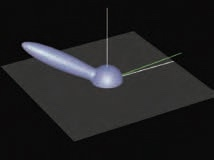
\includegraphics[width=1.\textwidth]{graphics/gi/ray-optics-8-2}
	\end{subfigure}
	\begin{subfigure}[b]{0.325\textwidth}
		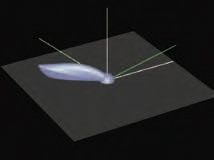
\includegraphics[width=1.\textwidth]{graphics/gi/ray-optics-8-3}
	\end{subfigure}
	\begin{subfigure}[b]{0.325\textwidth}
		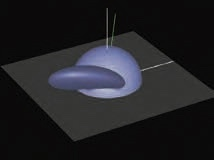
\includegraphics[width=1.\textwidth]{graphics/gi/ray-optics-8-4}
	\end{subfigure}
	\begin{subfigure}[b]{0.325\textwidth}
		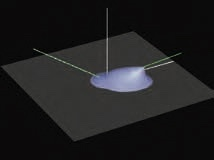
\includegraphics[width=1.\textwidth]{graphics/gi/ray-optics-8-5}
	\end{subfigure}
	\begin{subfigure}[b]{0.325\textwidth}
		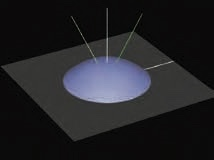
\includegraphics[width=1.\textwidth]{graphics/gi/ray-optics-8-6}
	\end{subfigure}
\end{center}
\caption{Example BRDF models. (Images courtesy of Szymon Rusinkiewicz, from his "bv" BRDF browser.)}
\end{figure}

Due to the non-optically smooth of surfaces, the microgeometry variation causes each surface point to reflect (and refract) light in a different direction, see figure \ref{f:microgeometry}. So for a given direction of incoming light, the BRDFs values are displayed for all outgoing directions. In figure \ref{f:brdf-models}, the spherical part around the point of intersection is the diffuse component, since outgoing radiance has an equal chance of reflecting in any direction. The ellipsoidal piece is a reflectance lobe, and is from the specular component.

Disney has a tool BRDF Explorer\footnote{\url{http://www.disneyanimation.com/technology/brdf.html}} which is an application that allows the development and analysis of BRDFs. It can load and plot analytic BRDF functions (coded as functions in OpenGL's GLSL shader language), measured material data from the MERL database, and anisotropic measured material data from MIT CSAIL. Graphs and visualizations update in realtime as parameters are changed, making it a useful tool for evaluating and understanding different BRDFs (and other component functions).


\subsubsection{Microfacet Specular BRDF}
Now we are going to derive the BRDF formulations. This subsection is for the specular BRDF, the next subsection is for the diffuse BRDF.

Microfacet theory is a way to derive BRDFs for surface reflection from non-optically flat surfaces. The assumption behind it is a surface with detail that is small compared to the scale of observation but large compared to a light wavelength. Each point is locally a perfect mirror, reflecting each incoming ray of light into one outgoing direction, which depends on the light direction $\mathbf{l}$ and the microfacet normal $\mathbf{m}$. 

In microfacet theory, a surface is characterized by the distribution of the microfacet surface normals. This distribution is defined by the surface's \textit{normal distribution function}, or NDF, we will see in this subsection. The NDF is defined as the probability distribution function of the microfacet surface normals. Most surfaces have NDFs that show a strong peak at the macroscopic surface normal $\mathbf{n}$.

Since each microfacet is assumed to be an ideal mirror, it reflects each incoming ray of light in a single reflected direction. So only those microfacets that happen to be oriented such that they reflect $\mathbf{l}$ into $\mathbf{v}$ can participate in the reflection, see figure \ref{f:microfacet}. This means that the participating or active microfacets have their surface normal aligned with a vector pointing exactly halfway between $\mathbf{l}$ and $\mathbf{v}$. This vector is called the \textit{half vector} $\mathbf{h}$.

\begin{figure}
\sidecaption
	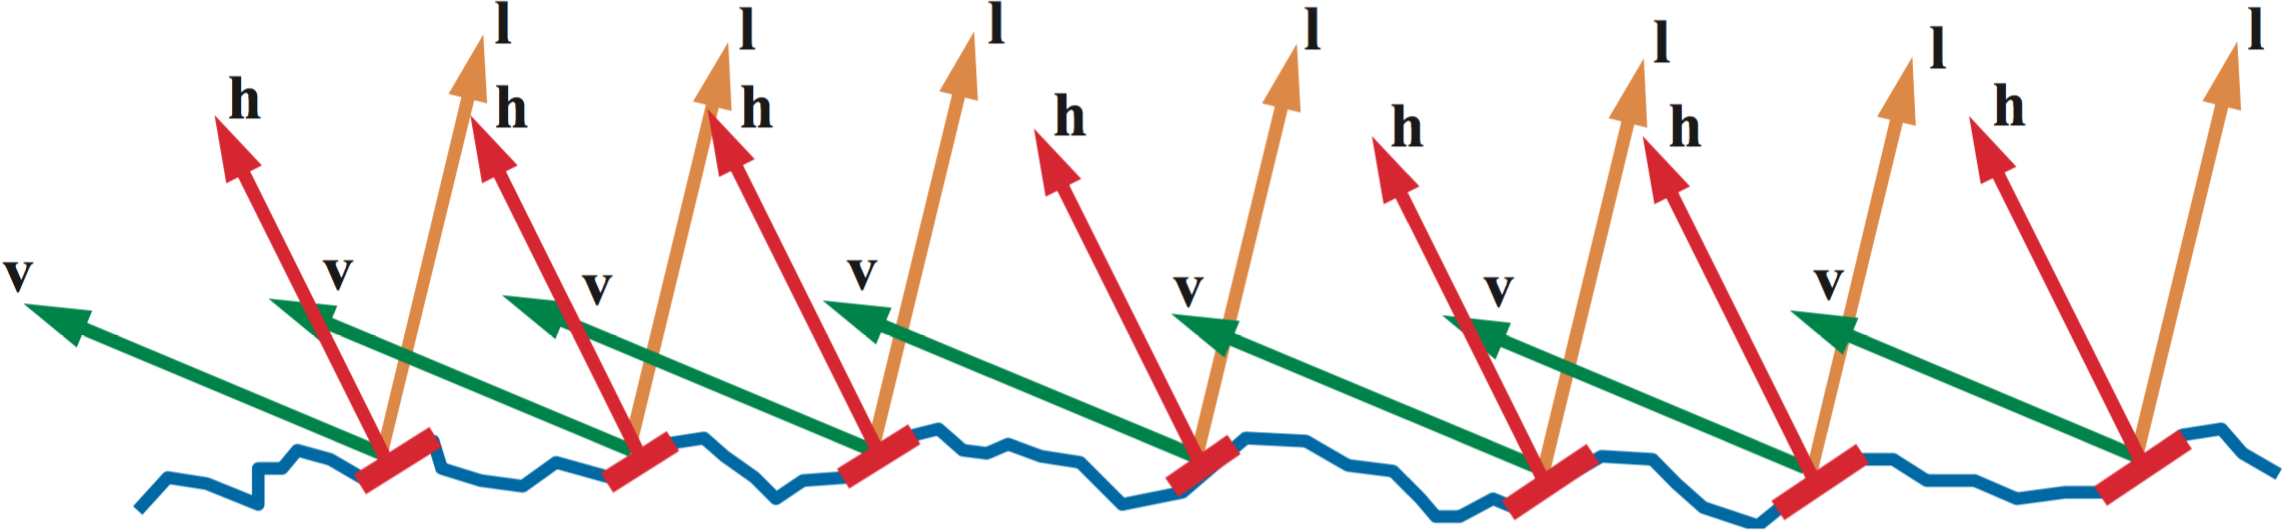
\includegraphics[width=.65\textwidth]{graphics/gi/ray-optics-9}
	\caption{Surface composed of microfacets. Only the red microfacets, which have their surface normal aligned with the half vector $\mathbf{h}$, participate in the reflection of light from the incoming light vector $\mathbf{l}$ to the view vector $\mathbf{v}$.}
	\label{f:microfacet}
\end{figure}

Not all microfacets with $\mathbf{m}=\mathbf{h}$ will contribute: some will be blocked by other microfacets from either light direction, see figure \ref{f:microfacet-effect}(a) or the view direction, see figure \ref{f:microfacet-effect}(b). In reality, blocked light continues to bounce; some will eventually contribute to the BRDF. Microfacet BRDFs ignore this, see figure \ref{f:microfacet-effect}(c), so effectively they assume all blocked light is lost.

\begin{figure}\label{f:microfacet-effect}
\begin{center}
	\begin{subfigure}[b]{0.34\textwidth}
		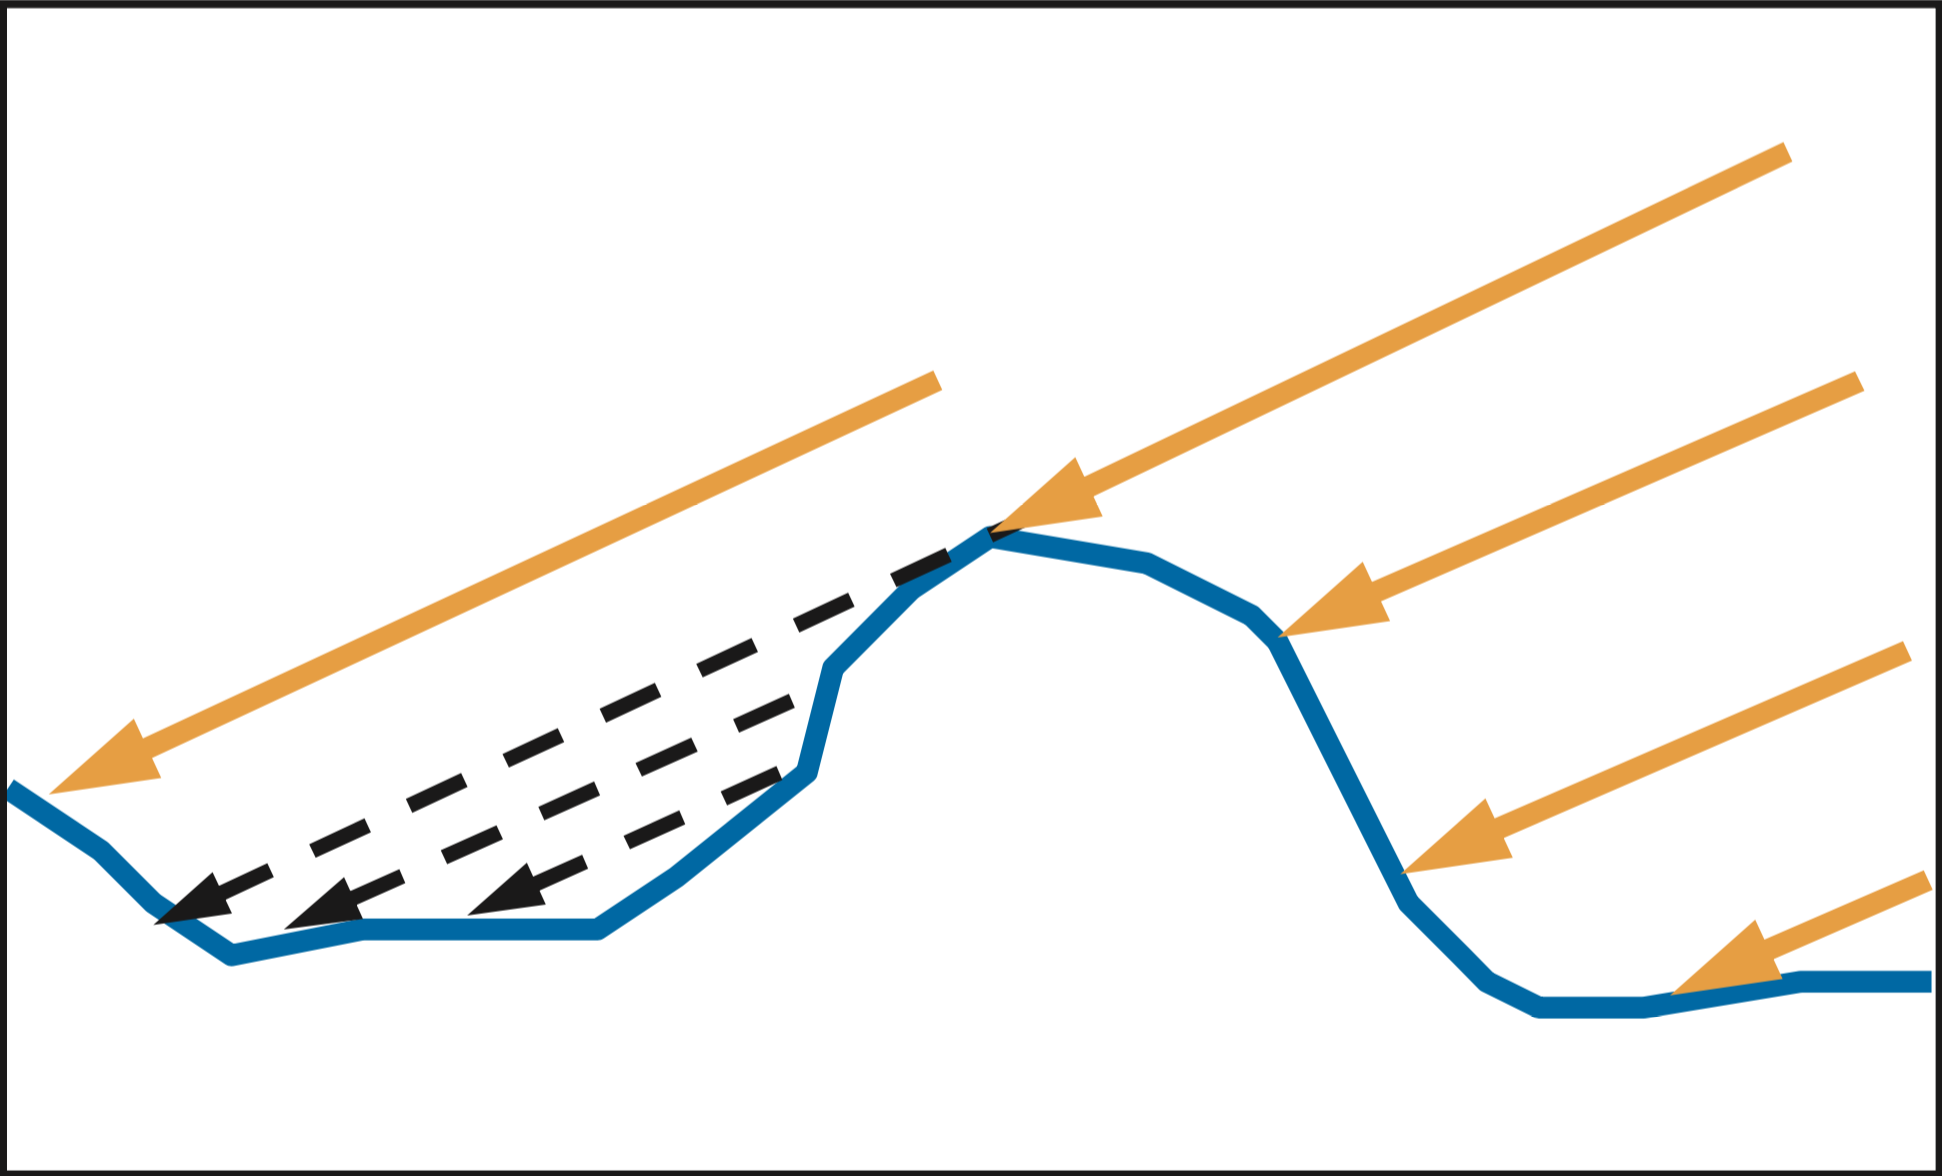
\includegraphics[width=1.\textwidth]{graphics/gi/ray-optics-10-1}
		\caption{Shadowing}
	\end{subfigure}
	\begin{subfigure}[b]{0.34\textwidth}
		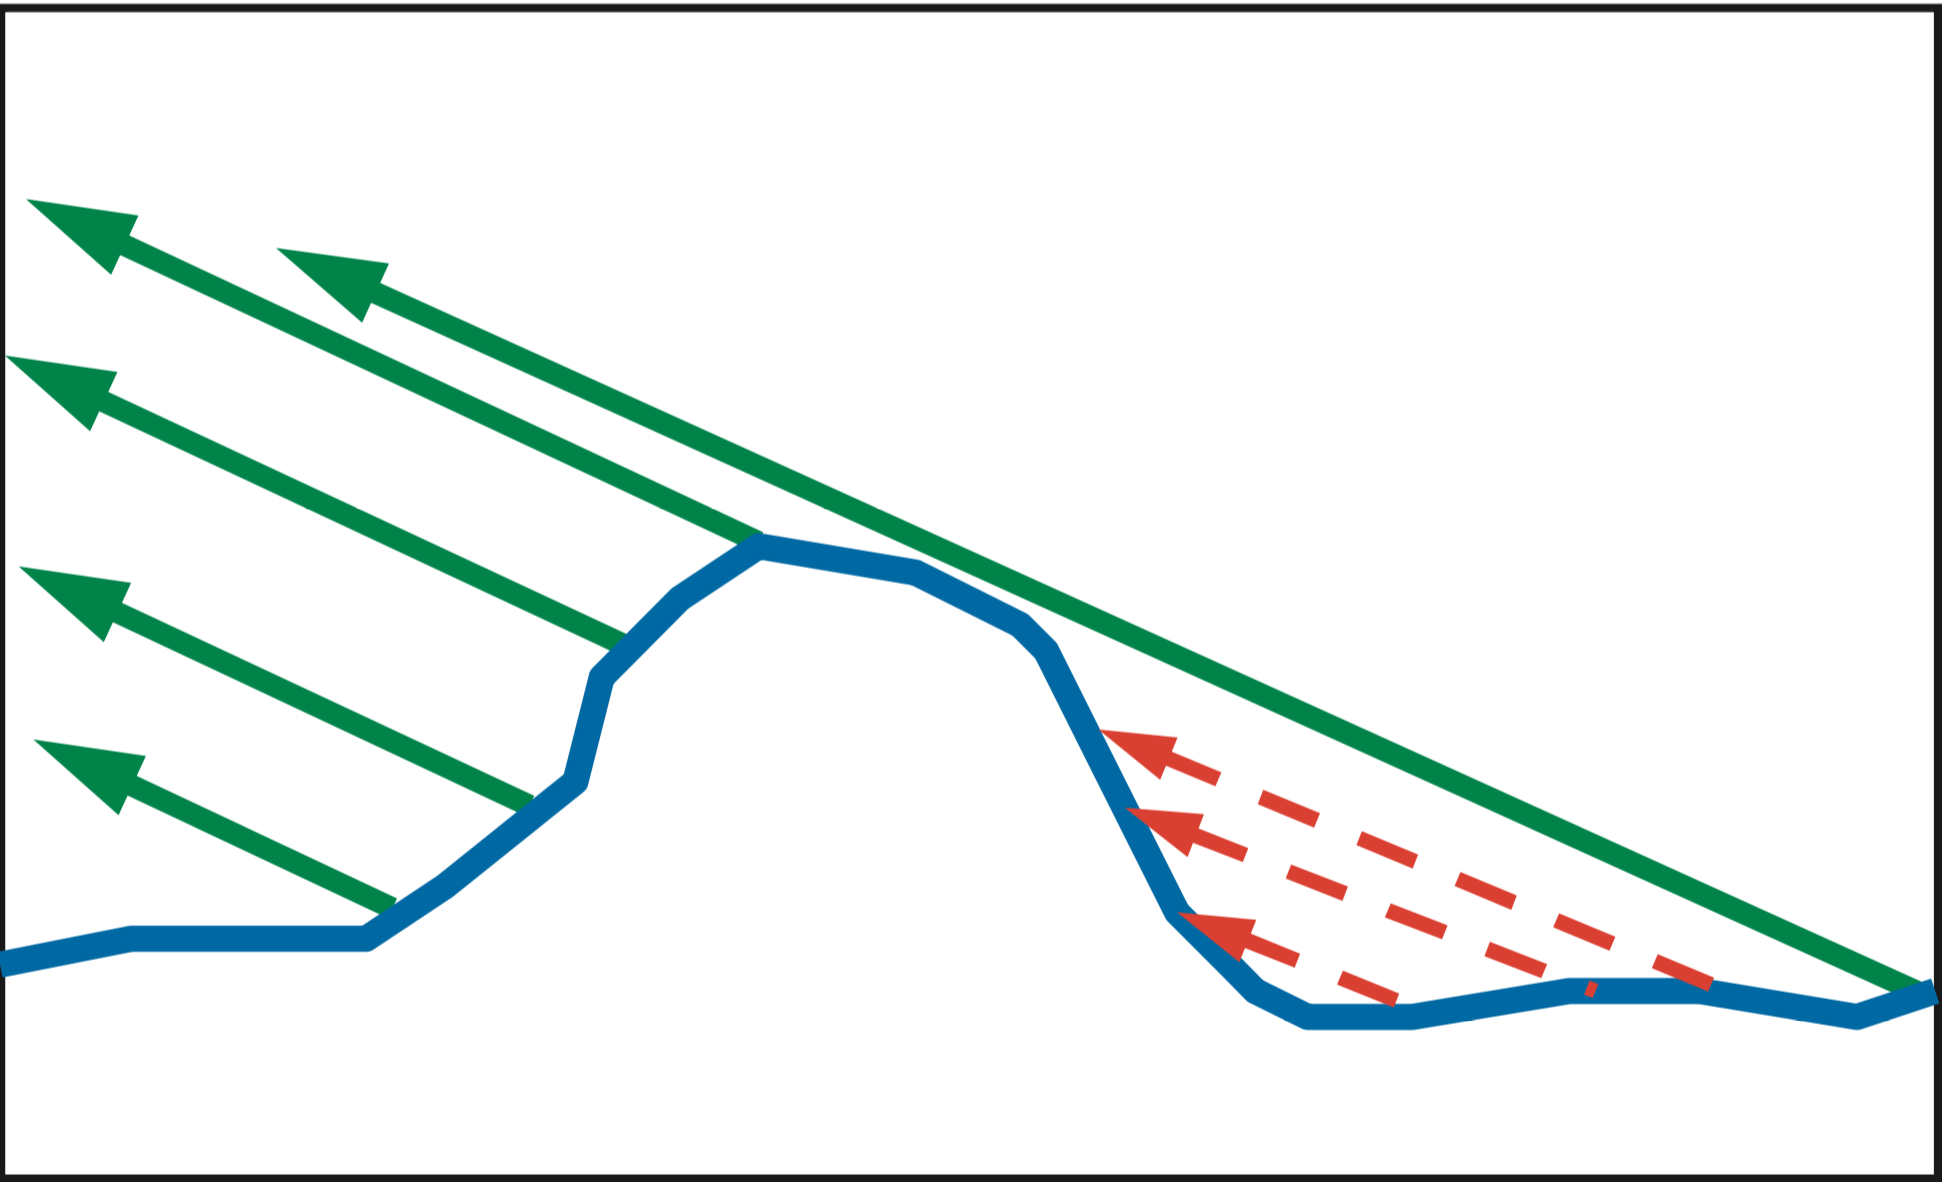
\includegraphics[width=1.\textwidth]{graphics/gi/ray-optics-10-2}
		\caption{Masking}
	\end{subfigure}
	\begin{subfigure}[b]{0.283\textwidth}
		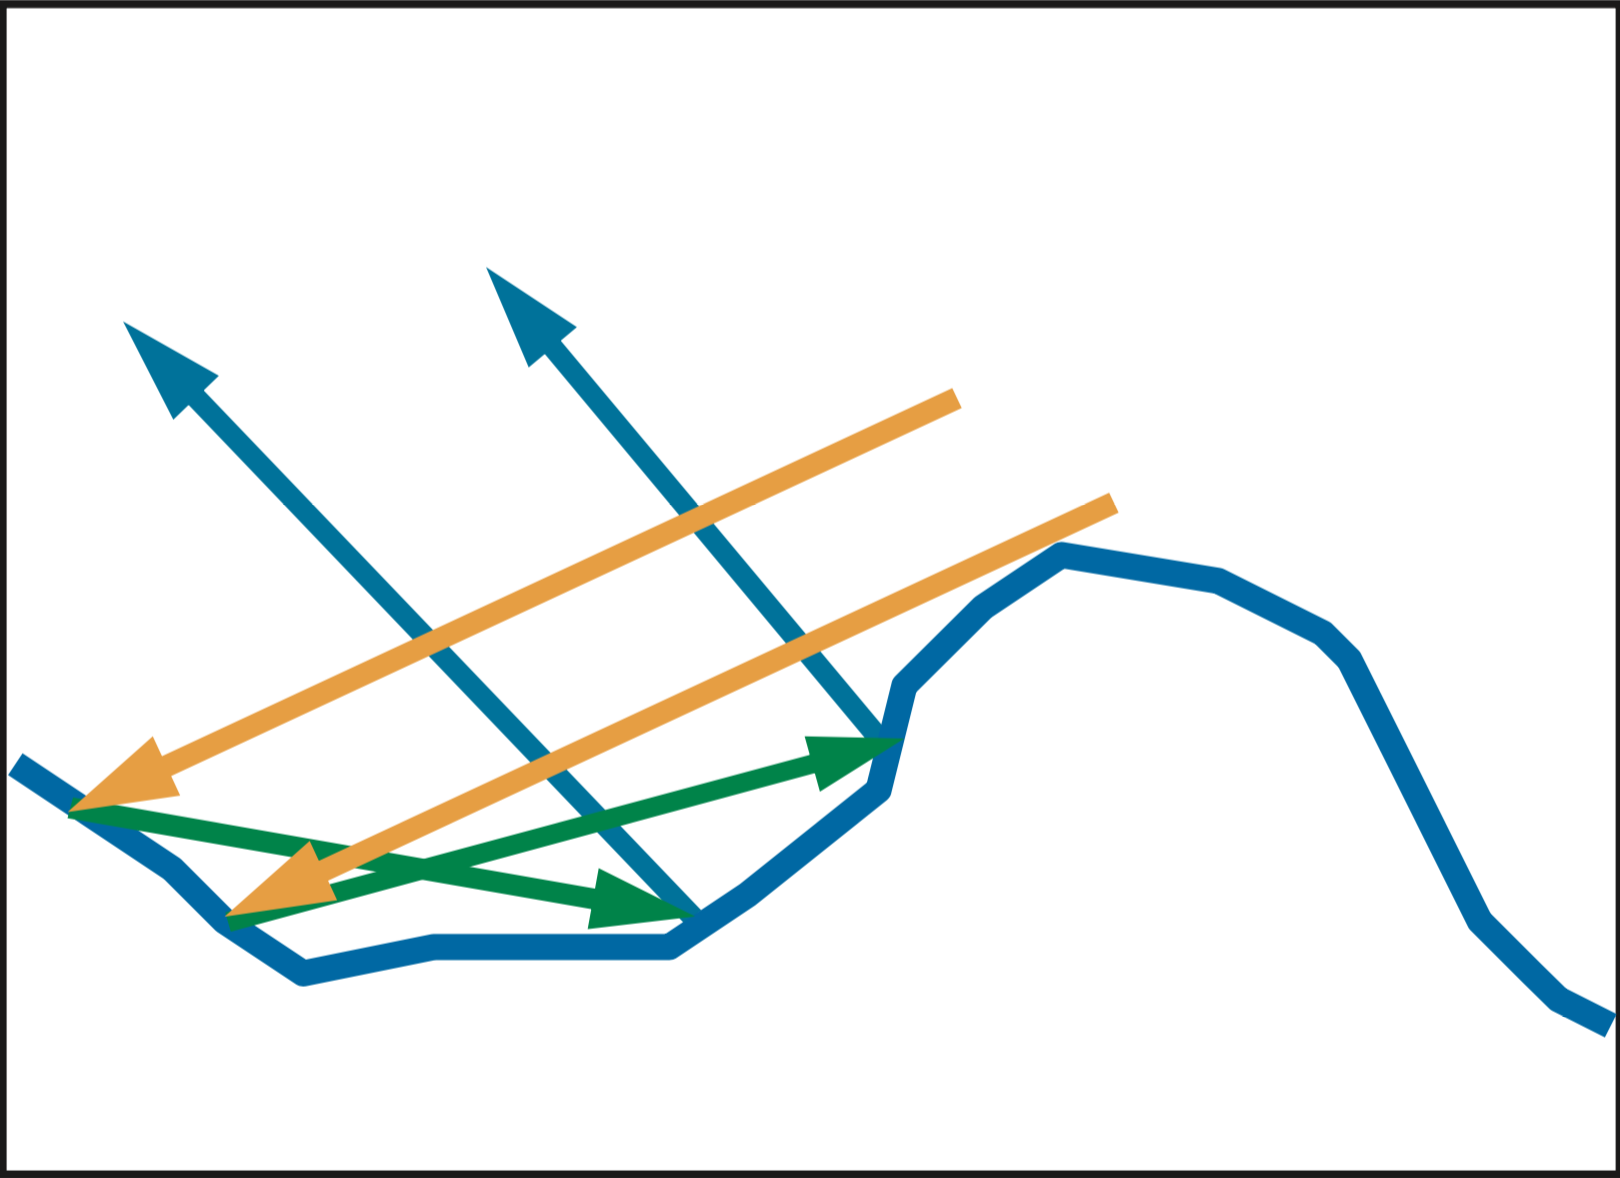
\includegraphics[width=1.\textwidth]{graphics/gi/ray-optics-10-3}
		\caption{Interreflection}
	\end{subfigure}
\end{center}
\caption{Geometrical effects of microscale structure. (a): the black dashed arrows indicate an area that is shadowed (occluded from the light) by other microgeometry. (b): the red dashed arrows indicate an area that is masked (occluded from view) by other microgeometry. (c): interreflection of light between the microscale structures is shown.}
\end{figure}

The general microfacet specular BRDF is:

\begin{equation}
	f(\mathbf{l},\mathbf{v})=\frac{F(\mathbf{l},\mathbf{h})G(\mathbf{l},\mathbf{v},\mathbf{h})D(\mathbf{h})}{4(\mathbf{n}\cdot\mathbf{l})(\mathbf{n}\cdot\mathbf{v})}
\end{equation}

This equation contains three part: fresnel reflection $F(\mathbf{l},\mathbf{h})$, geometry function $G(\mathbf{l},\mathbf{v},\mathbf{h})$ and  normal distribution function $D(\mathbf{h})$.

\begin{figure}
\sidecaption
	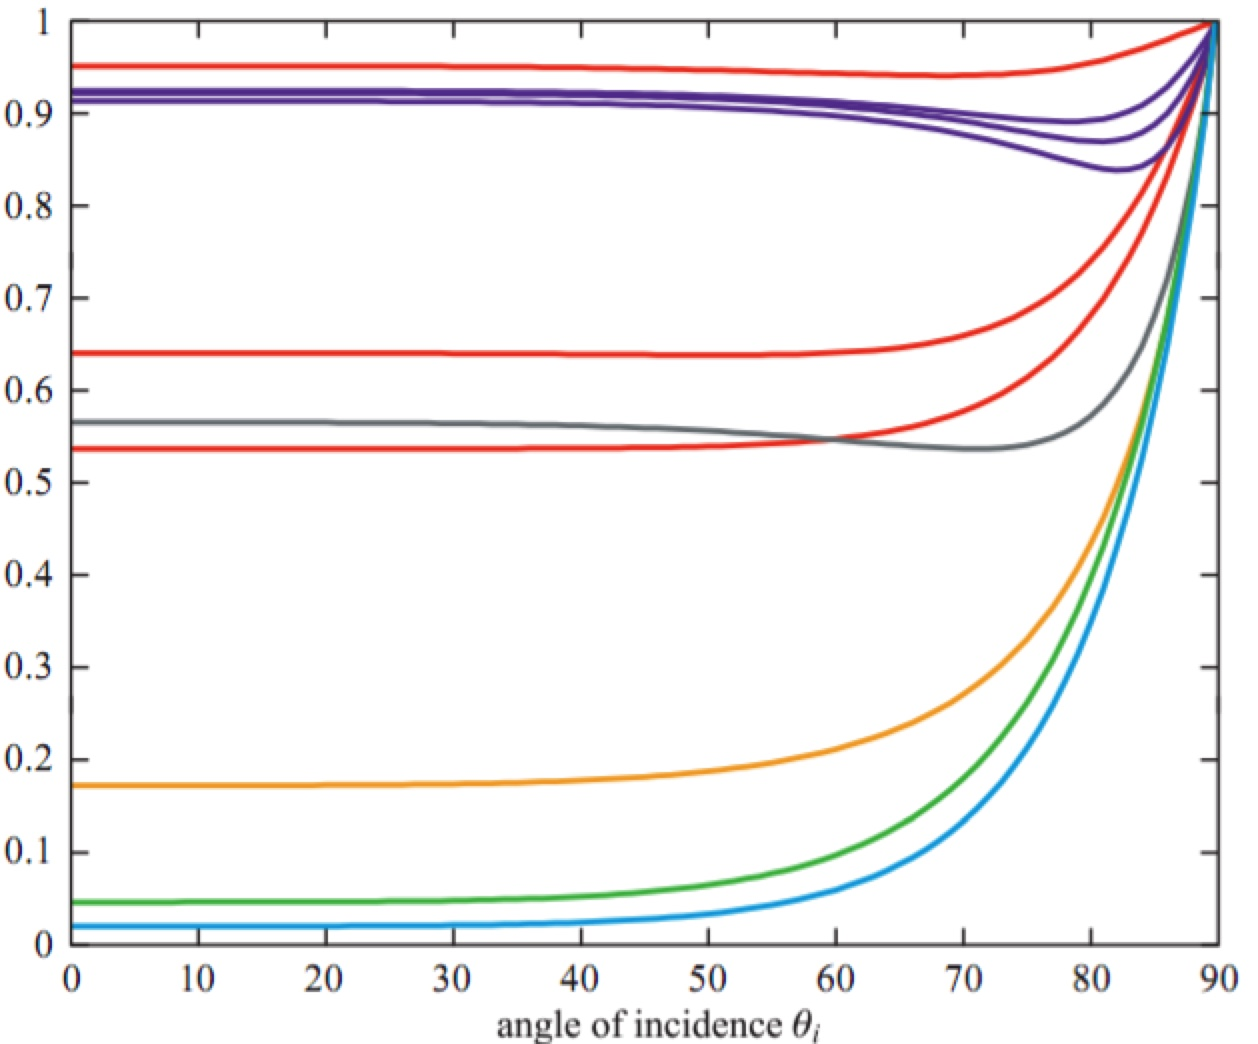
\includegraphics[width=.65\textwidth]{graphics/gi/ray-optics-11}
	\caption{Surface composed of microfacets. Only the red microfacets, which have their surface normal aligned with the half vector $\mathbf{h}$, participate in the reflection of light from the incoming light vector $\mathbf{l}$ to the view vector $\mathbf{v}$.}
	\label{f:Fresnel-reflection}
\end{figure}


\paragraph{\textbf{Fresnel reflectance}} $F(\mathbf{l},\mathbf{h})$, is the fraction of incoming light that is reflected (as opposed to refracted) from an optically flat surface of a given substance. It varies based on the light direction and the surface normal. Fresnel reflectance tells us how much of the light hitting the relevant microfacets (the ones facing in the half-angle direction) is reflected. see figure \ref{f:Fresnel-reflection}.

In the game industry the Schlick Fresnel approximation\cite[-5mm]{a:AnInexpensiveBRDFModelforPhysically-BasedRendering} is the most commonly used. It is cheap and reasonably accurate:

\begin{equation}
	F_{Schlick}=F_0 +(1-F_0)(1-cos\theta_d)^5
\end{equation}  

where the constant, $F_0$,  represents the specular reflectance at normal incident and achromatic for dielectrics and chromatic for metals. The actual value depends on the index of refraction, and $\theta_d$, the angle between the light vector $\mathbf{l}$ and the half vector $\mathbf{h}$. The effect of fresnel reflectance can be seen in figure \ref{f:fresnell-effect}.

\begin{figure}
\sidecaption
	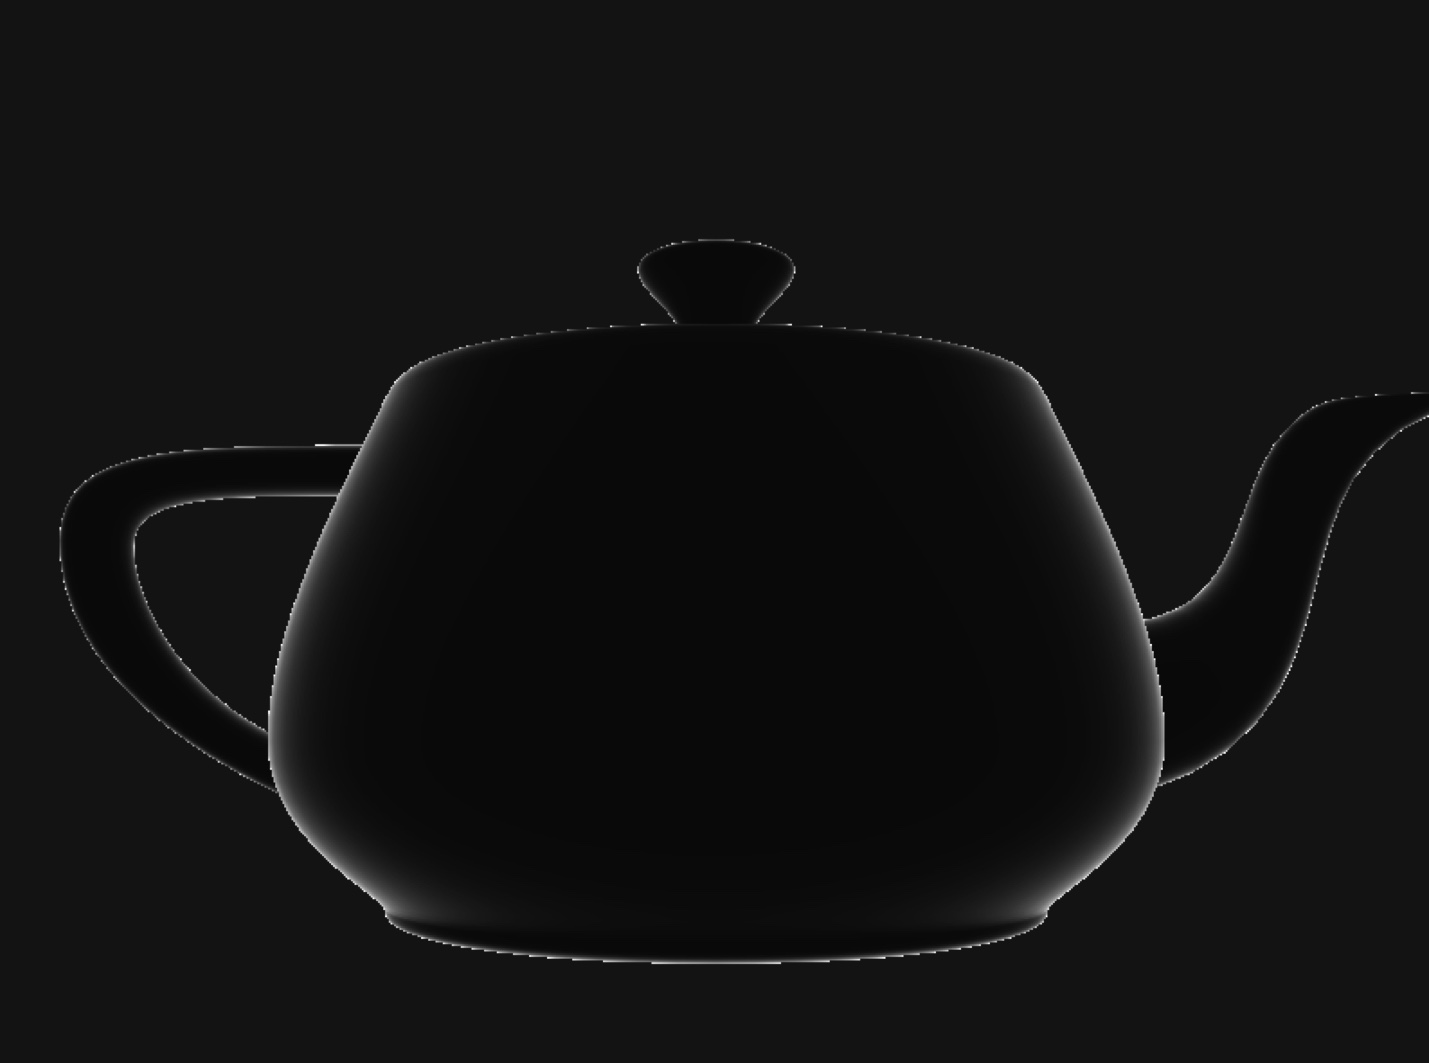
\includegraphics[width=.65\textwidth]{graphics/gi/ray-optics-12}
	\caption{This image shows the Fresnel reflectance of glass over a 3D shape. See how the dark reflectance color in the center brightens to white at the edges.}
	\label{f:fresnell-effect}
\end{figure}




\paragraph{\textbf{Normal distribution function}} $D(\mathbf{h})$, which gives the concentration of microfacet normals pointing in a given direction (half vector), relative to surface area. The NDF determines the size and shape of the highlight.

As the observations of Disney, the vast majority of the MERL\footnote{\url{http://www.merl.com/brdf/}} materials have specular lobs with tails that are much longer than traditional specular models. An example is the chrome sample shown in figure \ref{f:specular-lob-tails}. The specular response of this typical for smooth, highly polished surfaces, with a specular peak only a couple of degrees wide and a specular tails that is many times wider.

\begin{figure}\label{f:specular-lob-tails}
\begin{center}
	\begin{subfigure}[b]{0.3\textwidth}
		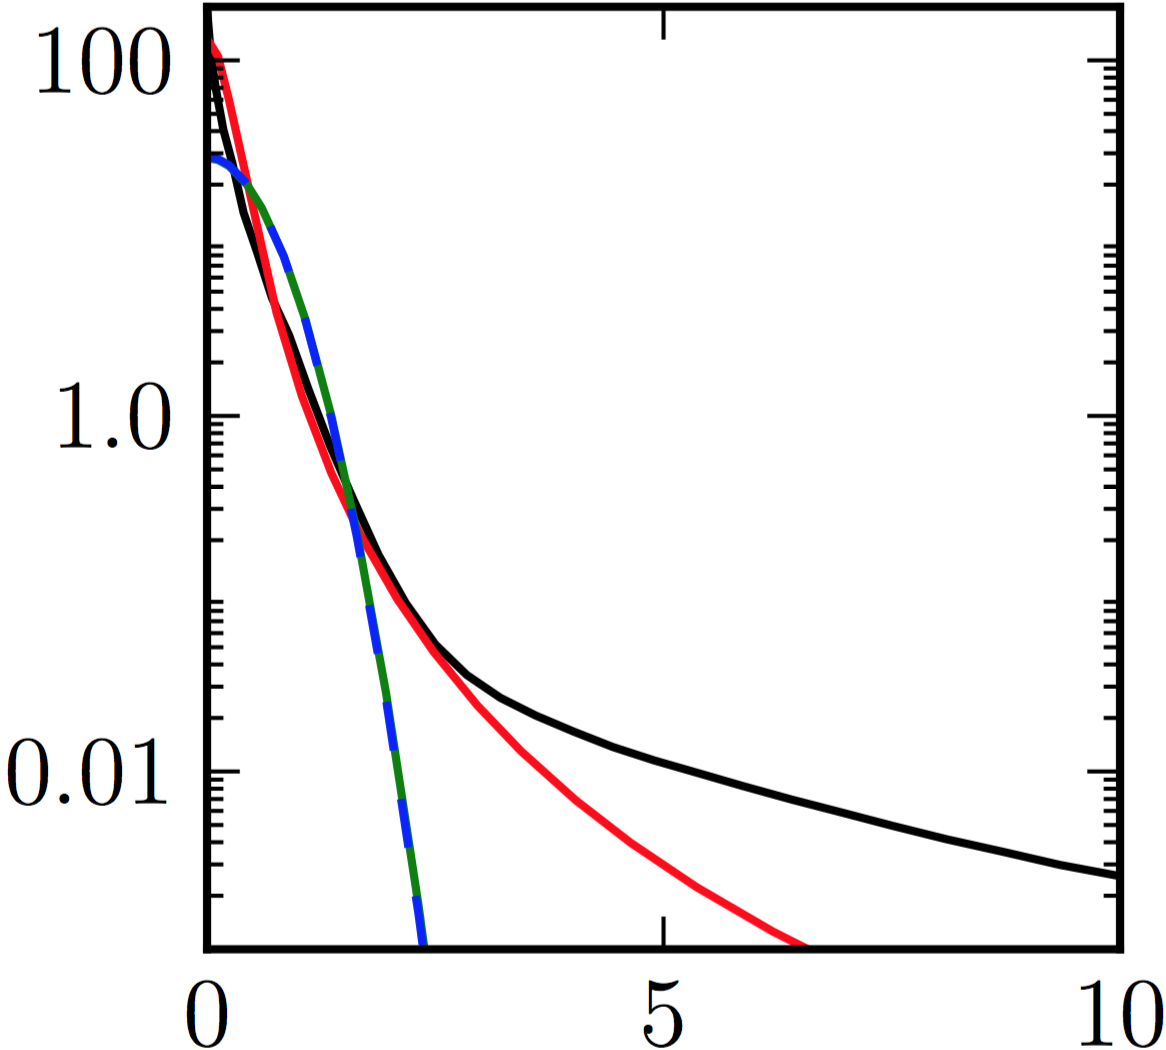
\includegraphics[width=1.\textwidth]{graphics/gi/ray-optics-13-1}
	\end{subfigure}
	\begin{subfigure}[b]{0.68\textwidth}
		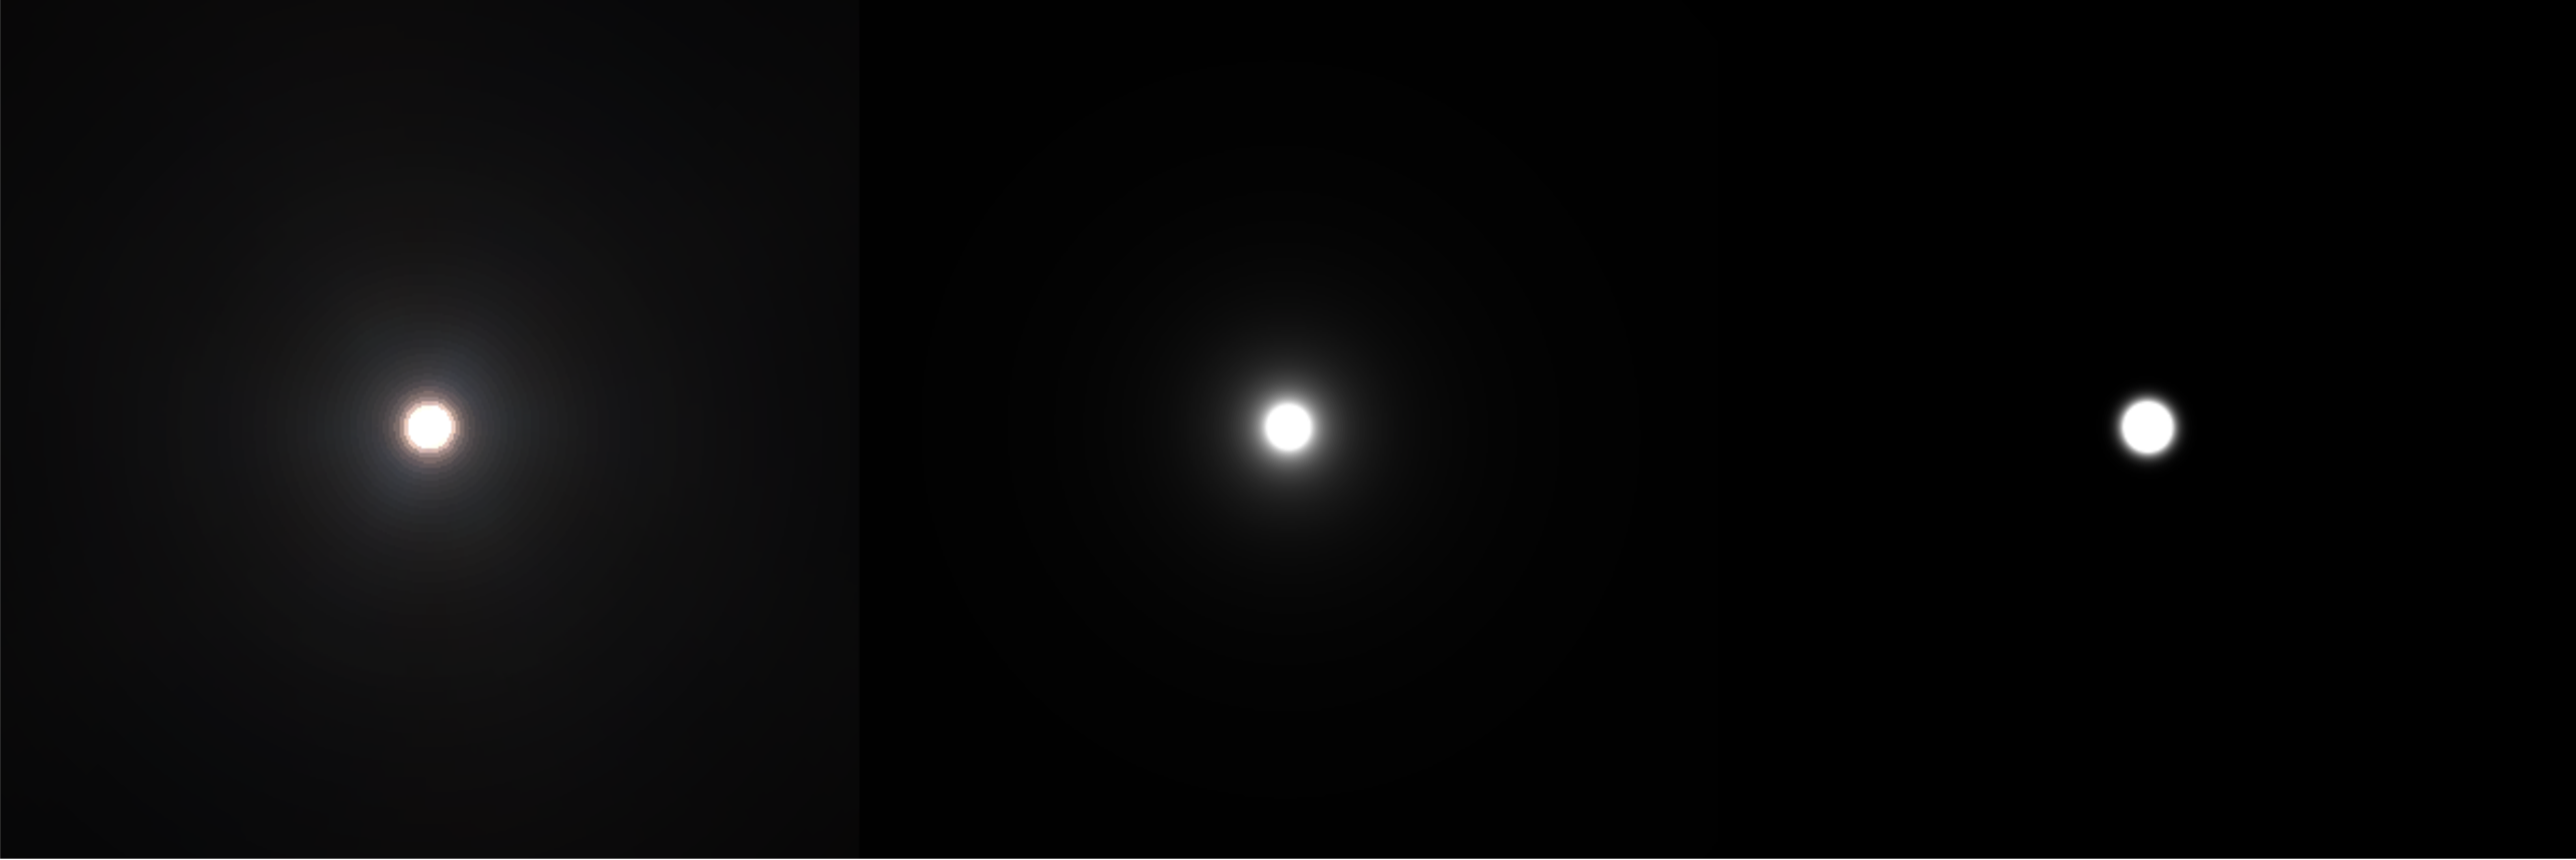
\includegraphics[width=1.\textwidth]{graphics/gi/ray-optics-13-2}
	\end{subfigure}
\end{center}
\caption{Several specular distributions fit to MERL chrome. Left: log-scale plots of specular peak vs $\theta_h$ (degrees); black = chrome, red = GGX ($\alpha$ = 0.006), green = Beckmann ($m$ = 0.013), blue = Blinn Phong ($n$ = 12000). Right: (clipped) point light responses from chrome, GGX, and Beckmann.}
\end{figure}

Disney choose the GGX/Trowbridge-Reitz, or GTR, algorithm:

\begin{equation}
	D_{GTR}(\mathbf{h})=\frac{\alpha^{2}}{\pi((\mathbf{n}\cdot\mathbf{h})^2 (\alpha^2-1)+1)^2}
\end{equation}

where $\alpha=roughness^2$ which we will introduce later on.

\paragraph{\textbf{Geometry function}} or shadow-masking function gives the chance that a microfacet with a given orientation is lit and visible from the given light and view directions.

In Unreal Engine 4\cite{a:RealShadinginUnrealEngine4}, they chose to use the Schlick model, but with $k=\alpha /2$. They also chose to use Disney's modification to reduce "hotness" by remapping roughness using $\frac{roughness+1}{2}$ before squaring. The final equation is:

\begin{equation}
	\begin{aligned}
		k&=\frac{(Roughness+1)^2}{8}\\
		G_1(\mathbf{v})&=\frac{\mathbf{n}\cdot\mathbf{v}}{(\mathbf{n}\cdot\mathbf{v})(1-k)+k}\\
		G(\mathbf{l},\mathbf{v},\mathbf{h})&=G_1(\mathbf{l})G_1(\mathbf{v})
	\end{aligned}
\end{equation}


\subsubsection{Diffuse BRDF}
For subsurface reflection -- diffuse term, the Lambert is the most common used in game and film production. It's the simplest possible BRDF: a constant value:

\begin{equation}
	f_{Lambert}(\mathbf{l},\mathbf{v})=\frac{c_{diff}}{\pi}
\end{equation}

where $c_{diff}$ is the diffuse albedo of material.

There are few important physical phenomena that Lambert doesn't account for. Since surface reflection goes to 100\% at glancing angles, it follows that diffuse should go to 0\%. Lambert also doesn't account for surface roughness. In most case, microscopic roughness affects specular. But some surface have microgeometry larger than the scattering distance, and these do affect diffuse reflectance.

Disney developed a novel empirical model\cite{a:PhysicallyBasedShadingatDisney} for diffuse is:

\begin{equation}
	f_d=\frac{baseColor}{\pi}(1+(F_{D90}-1)(1-cos\theta_l)^5)(1+(F_{D90}-1)(1-cos\theta_v)^5)
\end{equation} 

where $F_{D90}=0.5+2(roughness) cos^2\theta_d$.





\subsection{Material Model}
In rendering time, light interacts with surface. We've known how to represent the reflection distribution of the light, now we need to know how to represent the surfaces.

In computer graphics, the physical properties of the surface is stored in a called \textit{material} object, which also includes shaders. When rendering, these properties (i.e., roughness) and shaders, which includes the aforementioned functions, are submitted to GPU, and GPU uses these shaders and some light sources to compute the color of the point on the surface.

Here we introduce the Unreal Engine 4 material model\footnote{\url{https://docs.unrealengine.com/latest/INT/Engine/Rendering/Materials/PhysicallyBased/index.html}}. About material there are lots of topics, but we only discuss the properties relative to the functions we have introduced above, which is also called \textit{physically based materials} in Unreal Engine 4. This model is also a simplification of Disney's\cite{a:PhysicallyBasedShadingatDisney}.

In Unreal Engine 4, there are four properties deal with physically based shading:

\begin{itemize}
	\item Base Color
	\item Roughness
	\item Metallic
	\item Specular
\end{itemize}

All of these inputs are designed to taken in values between 0 and 1. In the case of Base Color, this means a color with RGN values that fall between 0 and 1. Physically based values can be measured from real world Materials.

\paragraph{\textbf{Base Color}} simply defines the overall color of the Material. It takes in a Vector3 (RGB) value and each channel is automatically clamped between 0 and 1.

\paragraph{\textbf{Roughness}} controls how rough the material is. A rough material will scatter reflected light in more directions than a smooth material. This can be seen in how blurry or sharp the reflection is or in how broad or tight the specular highlight is. Roughness of 0 (smooth) is a mirror reflection and roughness of 1 (rough) is completely matte or diffuse, see figure \ref{f:material-roughness}.

\begin{figure}\label{f:material-roughness}
\begin{center}
	\begin{subfigure}[b]{1.\textwidth}
		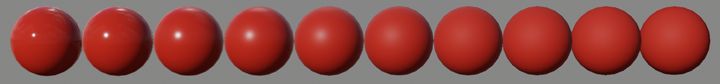
\includegraphics[width=1.\textwidth]{graphics/gi/roughness_nonmetal}
	\end{subfigure}
	\begin{subfigure}[b]{1.\textwidth}
		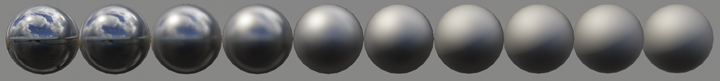
\includegraphics[width=1.\textwidth]{graphics/gi/roughness_metal}
	\end{subfigure}
\end{center}
\caption{Roughness 0 to 1. Nonmetal top, metal bottom.}
\end{figure}

We have seen that the roughness as a parameter for normal distribution function and geometry function in BRDF equation. Some game Engine (like Frostbite\cite{a:MovingFrostbitetoPBR}) chose \textit{smoothness} rather than roughness, because white = smooth is more intui1ve for them. 


\paragraph{\textbf{Metallic}} controls how "metal-like" your surface will be. Nonmetals have Metallic values of 0, metals have Metallic values of 1. For pure surfaces, such as pure metal, pure stone, pure plastic, etc. this value will be 0 or 1, not anything in between. When creating hybrid surfaces like corroded, dusty, or rusty metals, you may find that you need some value between 0 and 1.

\begin{figure}\label{f:material-metallic}
\sidecaption
	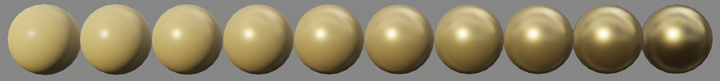
\includegraphics[width=1.\textwidth]{graphics/gi/metallic}
\caption{Metallic 0 to 1. Interpolating between two very different materials, shiny metallic gold and blue rubber.}
\end{figure}

For these values between 0 and 1, a interpolation method has been used. In Unreal Engine, layered materials\footnote{\url{https://docs.unrealengine.com/latest/INT/Engine/Rendering/Materials/LayeredMaterials/index.html}} can be used to blend two different materials.


\paragraph{\textbf{Specular}} is used to scale the current amount of specularity on non-metallic surfaces. It has no effect on metals.

Commonly, if we modify Specular, we do so to add micro occlusion or small scale shadowing, say from cracks represented in the normal map. These are sometimes referred to as cavities. Small scale geometry, especially details only present in the high poly and baked into the normal map, will not be picked up by the renderer's real-time shadows. To capture this shadowing, we generate a \textit{cavity map}, which is typically an AO map with very short trace distance. This is multiplied by the final BaseColor before output and multiplied with 0.5 (Specular default) as the Specular output. To be clear this is BaseColor = Cavity*OldBaseColor, Specular = Cavity*0.5.


\subsection{The Rendering Equation}
Radiance is the final quantity computed by the rendering process. We have been using the \textit{reflectance equation} to compute it:

\begin{equation}
	L_o(\mathbf{p},\mathbf{v})=\int_{\Omega}f(\mathbf{l},\mathbf{v})\otimes L_i(\mathbf{p},\mathbf{l})cos\theta_i d\omega_i
\end{equation}

where $L_o(\mathbf{p},\mathbf{v})$ is the outgoing radiance from the surface location $\mathbf{p}$ in the view direction $\mathbf{v}$; $\Omega$ is the hemisphere of directions above $\mathbf{p}$; $f(\mathbf{l},\mathbf{v})$ is the BRDF evaluated for $\mathbf{v}$ and the current incoming direction $\mathbf{l}$; $L_i(\mathbf{p},\mathbf{l})$ is the incoming radiance into $\mathbf{p}$ from $\mathbf{l}$; $\otimes$ is the piecewise vector multiplication operator; and $\theta_i$ is the angle between $\mathbf{l}$ and the surface normal $\mathbf{n}$. The integration is over all possible $\mathbf{l}$ in $\Omega$.

The reflectance equation is a restricted special case of the full \textit{rendering equation}, presented by Kajiya in 1986\cite{a:TheRenderingEquation}:

\begin{equation}
	L_o(\mathbf{p},\mathbf{v})=L_e(\mathbf{p},\mathbf{v})+\int_\Omega f(\mathbf{l},\mathbf{v})\otimes L_o(r(\mathbf{p},\mathbf{l}),-\mathbf{l})cos\theta_i d\omega_i
\end{equation}

where $L_e(\mathbf{p},\mathbf{v})$ is the emitted radiance from the surface location $\mathbf{p}$ in direction $\mathbf{v}$; $r(\mathbf{p},\mathbf{l})$ is called the \textit{ray casting function}. This function returns the location of the first surface point hit by a ray cast from $\mathbf{p}$ in direction $\mathbf{l}$, see figure \ref{f:ray-casting-function}.

\begin{figure}\label{f:ray-casting-function}
	\sidecaption
		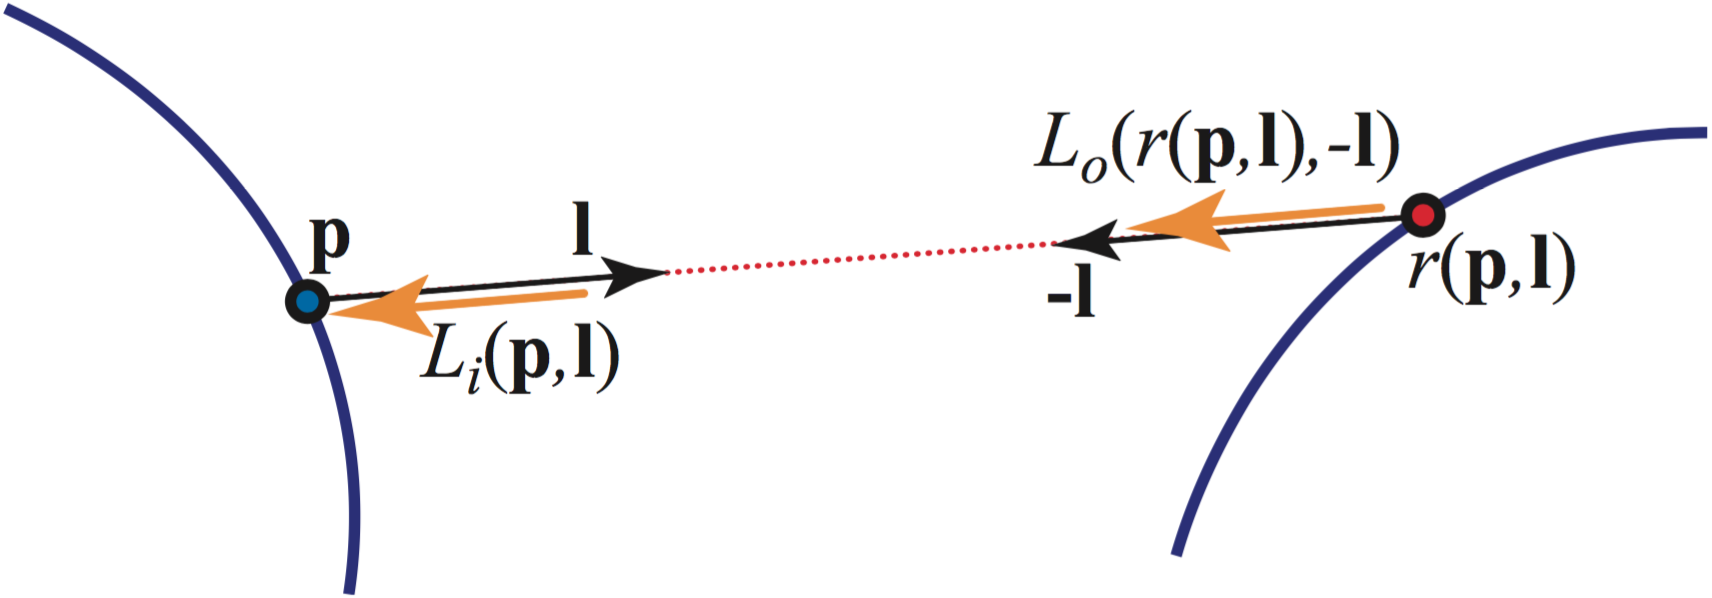
\includegraphics[width=0.65\textwidth]{graphics/gi/ray-optics-14}
	\caption{The shaded surface location $\mathbf{p}$, lighting direction $\mathbf{l}$, ray casting function $r(\mathbf{p}, \mathbf{l})$, and incoming radiance $L_i(\mathbf{p}, \mathbf{l})$, also represented as $L_o(r(\mathbf{p}, \mathbf{l}), −\mathbf{l})$.}
\end{figure}

$L_o(r(\mathbf{p},\mathbf{l}),-\mathbf{l})$ makes the rendering equation recursive. In order to compute the lighting at a surface we must solve for this recursive light energy distribution. In this article, we will introduce some methods to solve this cursive problem.

The rendering equation is very costly to compute and is far too complex to solve analytically in the general case. Because of this, it is typically approximated using numerical integration. Several algorithms have been proposed in the literature to fully or partially solve the rendering equation. These global illumination algorithms can generally be classified into two categories: finite element methods and Monte Carlo ray tracing methods.


%\section{Phenomena}
%\subsection{Ambient Occlusion}
%\subsection{Interreflections}
%\subsection{Reflections}
%\subsection{Caustics}
%\subsection{Subsurface Scattering}















